
\chapter[Applications of elliptic variational
  Inequality...]{Applications of elliptic variational Inequality
  methods to the solution of some nonlinear elliptic
  equations}\label{chap4} 

\section{Introduction}\label{c4:s1}

For\pageoriginale  solving some non-linear elliptic equations it may
be convenient, from the theoretical and numerical points of view, to
see them as EVI's. 

We shall consider in this chapter two examples of such situations:
\begin{enumerate}[(1)]
\item A family of mildly non-linear elliptic equations,
\item A non-linear elliptic equation modelling the subsonic flow of a
  perfect  compressible fluid. 
\end{enumerate}

\section[Theoretical and Numerical Analysis of...]{Theoretical and
  Numerical Analysis of Some\hfil\break Mildly Non-Linear Elliptic
  Equations}\label{c4:s2} 

\subsection{Formulation of the  continuous problem}\label{c4:ss2.1}

Let $\Omega$ be a bounded domain of $\mathbb{R}^N (N \geq 2)$ with a smooth boundary $\Gamma$. We consider 
\begin{itemize}
\item $V = H^1_0 (\Omega)$,
\item $L (v) = <f, v>$, $f \in V^* = H^{-1} (\Omega)$;
\item $a : V \times V \to \mathbb{R}$ bilinear, continuous and $V$-elliptic with $\alpha > 0$ as ellipticity constant; $a (\cdot, \cdot)$ is possibly not symmetric; 
\item $\phi : \mathbb{R} \to \mathbb{R}$, $\phi \in C^0 (\mathbb{R})$, non-decreasing with $\phi (0) = 0$.
\end{itemize}

We then consider the following non-linear elliptic equation $(P)$ defined by :

\textit{Find $u \in V$ such that}
\begin{equation}
\begin{cases}
a (u, v) + < \phi (u), v > = L (v) \ \forall v \in V,\\
\phi (u) \in L^1 (\Omega) \cap H^{-1} (\Omega). 
\tag{P}\label{c4:eqp} 
\end{cases}
\end{equation}

It follows from the \textit{Riesz representation Theorem} that there exists $A \in \mathscr{L} (V, V^*)$ such that $a (u, v) = <Au, v>\, \forall u, v \in V$. Therefore $(P)$ is equivalent to 
\begin{equation}
\begin{cases}
Au + \phi (u) = f, \\
u \in V,\\
\phi (u) \in L^1 (\Omega) \cap H^{-1} (\Omega). \tag{2.1}\label{c4:eq2.1}
\end{cases}
\end{equation}\pageoriginale 

\setcounter{example}{0}
\begin{example}\label{c4:exa2.1} %Exa 2.1
Let us consider a function $a_0 \in L^\infty (\Omega)$ such that 
\begin{equation}
a_0 (x) \geq \alpha > 0 \text{ a. e. in } \Omega. \tag{2.2}\label{c4:eq2.2}
\end{equation}
Define a $(\cdot , \cdot)$ by
\begin{equation}
a (u, v) = \int_\Omega a_0 (x) \nabla u \cdot \nabla v dx +\int_\Omega
\beta \cdot \nabla u vdx \tag{2.3}\label{c4:eq2.3} 
\end{equation}

where $\beta$ is a {\em constant} vector in $\mathbb{R}^N$.
\end{example}

From the definition of $a_0 (\cdot)$ and using the fact that $\int_\Omega \beta \cdot \nabla v vdx = 0\, \forall v \in H^1_0 (\Omega)$, we clearly have
\begin{equation}
a (v, v) \geq \alpha || v ||_V^2. \tag{2.4}\label{c4:eq2.4}
\end{equation}
From \eqref{c4:eq2.3} we obtain
\begin{equation}
Au = - \nabla \cdot (a_0 \nabla u) + \beta \cdot \nabla_u. \tag{2.5}\label{c4:eq2.5}
\end{equation}
Hence, in this particular case, \eqref{c4:eq2.1} becomes
\begin{equation}
\begin{cases}
- \nabla \cdot (a_0 \nabla u) + \beta \cdot \nabla u + \phi (u) = f, \\
u \in V, \phi (u) \in L^1 (\Omega). \tag{2.6}\label{c4:eq2.6}
\end{cases}
\end{equation}

\begin{remark}\label{c4:rem2.1}%Rem 2.1
If $N=1$, we have  $H^1_0 (\Omega) \subset C^0 (\overline{\Omega})$. Because of this inclusion there is no great difficulty in the study of one-dimensional problems of type $(P)$. If $N \geq 2$ the main difficulty is precisely related to the fact that $H^1_0 (\Omega)$ is not contained in $C^0 (\overline{\Omega})$.
\end{remark}

\begin{remark}\label{c4:rem2.2}%Rem 2.2
The analysis given below may be extended to problems in which either $V = H^1 (\Omega)$ or $V$  is a convenient closed subspace of $H^1(\Omega)$.
\end{remark}

\subsection{A variational inequality related to $(P)$}\label{c4:ss2.2}

\subsubsection {Definition of the variational 
inequality}\label{c4:sss2.2.1}\pageoriginale 

Let 
\begin{align}
& \Phi (t) = \int_0^t \phi (\tau) d \tau, \tag{2.7}\label{c4:eq2.7}\\
& D (\Phi) = \{v \in V : \Phi (v) \in L^1 (\Omega)\}.
\end{align}
The functional $j : L^2 (\Omega) \to \overline{\mathbb{R}}$ is defined by
\begin{equation}
j (v) = \int_\Omega \Phi (v) dx \text{ if } \Phi (v) \in L^1 (\Omega), j (v) = + \infty \text{ if } \Phi (v) \notin L^1 (\Omega).
\end{equation}
Instead of studying the problem $(P)$ directly, it is natural to associate to $(P)$ the following EVI of the second kind:
\begin{equation}
\begin{cases}
a (u, v-u) + j (v) -j (u) \geq L (v -u) \ \forall v \in V,\\
u \in V. \tag{$\pi$}
\end{cases}
\end{equation}

If $a (\cdot, \cdot)$ is symmetric, a standard method to study $(P)$ is to consider it as the \textit{formal Euler equation} of the following minimization problem encountered in the \text{Calculus of Variations}
\begin{equation}
\begin{cases}
J (u) \leq J (v) \ \forall v \in V, \\
u \in V, \tag{2.10}\label{c4:eq2.10}
\end{cases}
\end{equation}
where $J (v) = \frac{1}{2} a (v, v) + \int_\Omega \Phi (v) dx - L (v)$.

\begin{exercise}\label{c4:exer2.1}%Exe 2.1
Prove that $D (\Phi)$ is a convex, non-empty subset of $V$.
\end{exercise}

\subsubsection{Properties of $j (\cdot)$.}\label{c4:sss2.2.2} 	
Since $\phi : \mathbb{R} \to \mathbb{R}$ is non-decreasing and continuous with $\phi (0) = 0$, we have 
\begin{equation}
\Phi \in C^1 (\mathbb{R}), \Phi \text{ convex }, \Phi (0) = 0; \Phi (t) \geq 0\, \forall t \in \mathbb{R}.\tag{2.12}\label{c4:eq2.12}
\end{equation}

The properties of $j (\cdot)$ are given by the following

\begin{lemma}\label{c4:lem2.1}%Lem 2.1
The functional $j (\cdot)$ is convex, proper and 1.s.c. over $L^2(\Omega)$.
\end{lemma}

\begin{proof}
Since\pageoriginale  $j (v) \geq 0\, \forall \in L^2 (\Omega)$ it following that $j (\cdot)$ is proper. The convexity of $j (\cdot)$ is obvious from the  fact that $\Phi$ is convex.

Let us prove that $j (\cdot)$ is l.s.c. Let $(v_n)_n$, $v_n \in L^2 (\Omega)$ be such that
$$
\lim_{n \to \infty} v_n = v \text{ strongly in } L^2 (\Omega).
$$
Then we have to prove that
\begin{equation}
\liminf_{n \to \infty} j (v_n) \geq j (v). \tag{2.13}\label{c4:eq2.13}
\end{equation}
\end{proof}

If $\liminf \limits_{n \to \infty} j (v_n) = + \infty$ the property is proved. Therefore assume that $\liminf\limits_{ n \to \infty} j (v_n) = \ell < \infty$. Hence we can extract a subsequence $(v_{n_{k}})_n{_k}$ such that  
\begin{align}
& \lim_{k \to \infty} j (v_{n_k}) = \ell, \tag{2.14}\label{c4:eq2.14}\\
& v_{n_k} \to v \text { a. e. in } \Omega. \tag{2.15}\label{c4:eq2.15}
\end{align}
Since $\Phi \in C^1 (\mathbb{R})$, \eqref{c4:eq2.15} implies 
\begin{equation}
\lim_{k \to \infty} \Phi (v_{n_k}) = \Phi (v) ~\text{a.e.}. \tag{2.16}\label{c4:eq2.16}
\end{equation} 
Moreover $\Phi (v) \geq 0$ a.e and \eqref{c4:eq2.14} implies that
\begin{equation}
\{\Phi (v_{n_k})\}_k \text{ is bounded in } L^1 (\Omega). \tag{2.17}\label{c4:eq2.17}
\end{equation}
Hence by Fatou's Lemma, from \eqref{c4:eq2.16} and \eqref{c4:eq2.17}, we have
\begin{equation}
\begin{cases}
\Phi (v) \in L^1 (\Omega), \\
\liminf\limits_{k \to \infty} \int_\Omega \Phi (v_{n_k}) dx \geq \int_\Omega 
\Phi (v) dx. \tag{2.18}\label{c4:eq2.18}
\end{cases}
\end{equation}
From \eqref{c4:eq2.14} and \eqref{c4:eq2.18} we obtain \eqref{c4:eq2.13}. This  proves the lemma.

\setcounter{corollary}{0}
\begin{corollary}\label{c4:cor2.1}
The functional $j (\cdot)$ restricted to $V$ is convex, proper, l,s.c.
\end{corollary}

\subsubsection{Existence and uniqueness results for $(\pi)$ 
:}\label{c4:sss2.2.3}

\begin{theorem}\label{c4:thm2.1} %theorem 2.1
Under\pageoriginale  the above hypothesis on $V$, $a (\cdot, \cdot)$, $L (\cdot)$, $\phi (\cdot)$ the problem $(\pi)$ has a unique solution in $V \cap D (\phi)$.
\end{theorem}

\begin{proof}
Since $V$, $a (\cdot, \cdot)$, $L(\cdot)$, $j (\cdot)$ have the 
properties (cf. Corollary \ref{c4:cor2.1}) required to apply Theorem 
\ref{c1:thm4.1} of Chap.~\ref{chap1}, Sec.~\ref{c1:s4}, the EVI of the
second kind $(\pi)$, has a unique solution $u$ in $V$. 
\end{proof}

Let us show that $u \in D (\Phi)$. Taking $v = 0$ in $(\pi)$ we obtain
\begin{equation}
a (u, u) + j (u) \leq L (u) \leq || f || \cdot || u ||_V.
\end{equation}
Since $j (u) \geq 0$, using the ellipticity of $a (\cdot, \cdot)$ we obtain
\begin{equation}
|| u ||_V \leq \frac{|| f ||}{\alpha}, \tag{2.20}\label{c4:eq2.20}
\end{equation}
which implies
\begin{equation}
j (u) \leq \frac{|| f ||^2} {\alpha}. \tag{2.21}\label{c4:eq2.21}
\end{equation}
This implies $u \in D (\Phi)$. 

\begin{remark}\label{c4:rem2.3}%Rem 2.3
If $a (\cdot , \cdot)$ is symmetric, $(\pi)$ is equivalent to \eqref{c4:eq2.10}.
 \end{remark} 

\subsection{Equivalence between $(P)$ and $(\pi)$}\label{c4:ss2.3} 
In this section we shall prove that $(P)$ and $(\pi)$ are equivalent. First we prove that the unique solution of $(\pi)$ is also a solution of $(P)$. In order to prove this result we need to prove that $\phi (u)$ and $u \phi (u)$ belong  to $L^1 (\Omega)$.
 
\begin{proposition}\label{c4:prop2.1}%Pro 2.1
Let $u$ be the solution of $(\pi)$. Then $u \phi (u)$ and $\phi (u)$ belong to $L^1 (\Omega)$. 
 \end{proposition}

 \begin{proof}
Here we use a {\em truncation} technique. Let $n$ be a positive integer. Define
$$
K_n \{ v \in V : |v (x)| \leq n a.e. \}.
$$
 Since $K_n$ is a closed, convex, non-empty subset of $V$, the following variational inequality
 \begin{equation}
\begin{cases}
a (u^n, v-u^n) + j (v) - j (u^n) \geq L (v -u^n) \ \forall v \in K_n,\\
u^n \in K_n \tag{$\pi_n$}
\end{cases}
 \end{equation}\pageoriginale 
 has a unique solution (in order to apply Theorem \ref{c1:thm4.1} of 
 Chapter~\ref{chap1}, we need to replace $j$ by $j+I_{k_n}$ where $I_k$ is the \textit{indicator functional} of $K_n$).
   
Now we prove that $\lim\limits_{n \to \infty} u_n = u$ \textit{weakly} 
in $V$, where $u$ is the solution of $(\pi)$. Since $ 0 \in K_n$, 
taking $v = 0$ in $(\pi_n)$ we obtain as in Theorem \ref{c4:thm2.1} of this chapter that
 \begin{align}
& || u_n ||_V \leq \frac{||f||}{\alpha}. \tag{2.22}\label{c4:eq2.22}\\
& j (u_n) \leq \frac{|| f ||^2}{\alpha}. \tag{2.23}\label{c4:eq2.23}
\end{align} 
 
It follows from \eqref{c4:eq2.22} that there exists a subsequence $\{u_{n_k}\}$ of $(u_n)_n$ and $a u^* \in V$ such that
 \begin{equation}
\lim_{k \to \infty} u_{n_k} = u^* \text{ weakly in } V. \tag{2.24}\label{c4:eq2.24} 
 \end{equation} 
 Moreover, from the compactness of the canonical injection from $H^1_0 (\Omega)$ to $L^2 (\Omega)$ and form \eqref{c4:eq2.24}, it follows that
 \begin{equation}
\lim_{k \to \infty} u_{n_k} = u^* \text{ strongly in } L^2
(\Omega).\tag{2.25}\label{c4:eq2.25} 
\end{equation} 
 Relation \eqref{c4:eq2.25} implies that we can extract a subsequence,
 still denoted by $(u_{n_k})_{n_k}$, such that 
 \begin{equation}
\lim_{k \to \infty} u_{n_k} = u^* \text{ a. e. in } \Omega. \tag{2.26}\label{c4:eq2.26}
 \end{equation} 
 
Now let $v \in V \cap L^\infty (\Omega)$; then, large $k$, have $v \in K_{n_k}$ and
 \begin{equation}
a (u_{n_k}, u_{n_k}) + j (u_{n_k}) \leq a (u_{n_k}, v) + j (v) -L (v-u_{n_k}). \tag{2.27}\label{c4:eq2.27}
 \end{equation} 
 Since $\liminf\limits_{k \to \infty} a (u_{n_k}, u_{n_k}) \geq a (u^*, u^*)$ and $\liminf\limits_{k \to \infty} j (u_{n_k}) \geq j (u^*)$ it follows from\pageoriginale   \eqref{c4:eq2.24} and \eqref{c4:eq2.27} that
 \begin{equation*}
\begin{cases}
a (u^*, u^*) + j (u^*) \leq (u^*, v) +j(v) -L (v-u^*) \ \forall v \in L^\infty (\Omega) \cap V, \\
u^* \in V,
\end{cases}
\end{equation*} 
 which can also be written as 
 \begin{equation}
\begin{cases}
a (u^*, v-u^*) + j (v) -j (u^*) \geq -L (v-u^*) \ \forall v \in  V \cap L^\infty (\Omega), \\
u^* \in V. \tag{2.28}\label{c4:eq2.28}
\end{cases}
 \end{equation} 

 For $n > 0$, define $\tau_n : V \to K_n$ by
 \begin{equation}
\tau_n v =\inf (n, \Sup (-n, v)) (\text{ see Figure  \ref{c4:fig2.1}})
\tag{2.29}\label{c4:eq2.29} 
 \end{equation} 

\begin{figure}[H]
  \centering{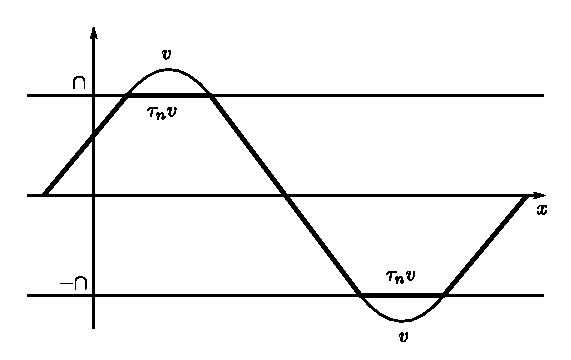
\includegraphics{vol65-figures/fig65-chap2.1.eps}}
  \caption{}\label{c4:fig2.1}
\end{figure}

Then the Corollary \ref{c2:cor2.1} of Chap.~\ref{chap2}, 
Sec.~\ref{c2:ss2.2}, we have
 \begin{equation}
\begin{cases}
\lim\limits_{n \to \infty} \tau_n v = v \text{ strongly in } V, \\
\lim\limits_{n \to \infty} \tau_n v = v \text{ in } \Omega. \\
\end{cases}\tag{2.30}\label{c4:eq2.30}
 \end{equation} 
 Moreover, we obviously have,
 \begin{align}
& |\tau_n v (x) | \leq | v (x) | ~\text{a.e.,} \tag{2.31}\label{c4:eq2.31}\\
& v (x) \cdot \tau_n v (x) \geq 0 ~\text{a.e.} \tag{2.32}\label{c4:eq2.32}
 \end{align}\pageoriginale 
It follows then from \eqref{c4:eq2.30}-\eqref{c4:eq2.32} and from the various properties of that
 \begin{align}
& \Phi (\tau_n v) \leq \Phi (v) ~\text{a.e.,} \tag{2.33}\label{c4:eq2.33}\\
& \lim_{n \to \infty} \Phi (\tau_n v) = \Phi (v) ~\text{a.e.} \tag{2.34}\label{c4:eq2.34}
 \end{align} 
 
 Since $\tau_n v \in L^\infty (\Omega) \cap V$ it follows form \eqref{c4:eq2.28} that
 \begin{equation}
\begin{cases}
a (u^*, \tau_n v - u^*) + j (\tau_n v) - j (u^*) \geq L (\tau_n v - u^*) \ \forall v \in V, \\
u^*  \in V. \tag{2.35}\label{c4:eq2.35}
\end{cases}
 \end{equation}
 If $v \notin D (\Phi)$, then by Fatou's lemma 
$$
\lim_{n \to \infty} j (\tau_n v) = + \infty.
$$
If $v \in D (\Phi)$, it follows from \eqref{c4:eq2.33} and
\eqref{c4:eq2.34} by applying Lebesgue's dominated convergence theorem
that 
$$
\lim_{n \to \infty} j (\tau_n v) = j (v).
$$
From these convergence properties and from \eqref{c4:eq2.30}, it follows, by taking the limit in \eqref{c4:eq2.35}, that
 \begin{equation}
\begin{cases}
a (u^*, v - u^*) + j (v) -j (u^*) \geq L (v -u^*) \ \forall v \in V,\\
u^* \in V. \tag{2.36}\label{c4:eq2.36}
\end{cases}
 \end{equation}
 
Then $u^*$ is a solution of $(\pi)$ and from the uniqueness property
we have $u^* = u$. This proves that $\lim\limits_{n \to \infty} u_n =
u$ \textit{weakly} in $V$.   
 
Let us know that $\phi (u)$, $u \phi (u) \in L^1 (\Omega)$. Let $v \in
K_n$. Then $u_n + t (v-u_n) \in K_n\, \forall t \in] 0,
  1]$. Replacing\pageoriginale  $v$ by $u_n + t (v-u_n)$ in $\pi_n$
    and dividing both sides of the inequality by $t$ we obtain  
 \begin{equation}
a (u_n, v-u_n) + \int_\Omega \frac{\Phi (u_n + t (v - u_n)) -\Phi (u_n)} {t} dx \geq L (v-u_n) \ \forall v \in K_n. \tag{2.37}\label{c4:eq2.37}
 \end{equation} 
Since  $\Phi \in C^1 (R)$ and $\Phi' = \phi$ we have
 \begin{equation}
\lim_{\substack{t \to 0\\{t >0}}} \frac{\Phi (u_n + t (v-u_n)) - \Phi
  (u_n)} {t} = \phi (u_n) \cdot (v-u_n)
~\text{a.e.}\tag{2.38}\label{c4:eq2.38}  
 \end{equation} 
 Moreover since $\Phi$ is convex, we also have $\forall t \in ] 0, 1]$,
 \begin{equation}
\phi (u_n) (v-u_n) \leq \frac{\phi (u_n + t (v - u_n)) -\phi (u_n)} {t} 
\leq \Phi (v) -\Phi (u_n) ~\text{a.e.} \tag{2.39}\label{c4:eq2.39} 
 \end{equation} 
 
 From \eqref{c4:eq2.38}, \eqref{c4:eq2.39} and using
 \textit{Lebesgue's dominated convergence Theorem} in
 \eqref{c4:eq2.37}, we obtain 
 \begin{equation}
a (u_n, v-u_n)+ \int_\Omega \phi (u_n) (v-u_n) dx \geq L (v-u_n) \quad
\forall v \in K_n.\tag{2.40}\label{c4:eq2.40} 
 \end{equation} 
Then taking  $v= 0$ in \eqref{c4:eq2.40} we have
 $$
 a (u_n, u_n) + \int_\Omega \phi (u_n) u_n dx \leq L (u_n),
 $$
 which implies, using \eqref{c4:eq2.2},
 \begin{equation}
\int_\Omega \phi (u_n) u_n dx \leq \frac{||f||^2}
    {\alpha}.\tag{2.41}\label{c4:eq2.41} 
 \end{equation} 
But $\phi (v) v \geq 0\, \forall v \in V$. Hence $\phi (u_n) u_n$ is bounded in $L^1 (\Omega)$. Moreover for some subsequence $(u_{n_k})_{n_k}$ of $(u_n)_n$ we have
 $$
 \phi (u_{n_k}) u_{n_k} \to \phi (u)u \text{ a. e. in } \Omega. 
 $$
Then by Fatou's lemma we obtain $u \phi (u) \in L^1 (\Omega)$ and this completes the proof of the Proposition since $u \phi (u) \in L^1 (\Omega)$ implies obviously that $\phi (u) \in L^1 (\Omega)$.
 \end{proof}

 Incidentally,\pageoriginale when proving the convergence of $(u_n)_n$ to $u$, we have proved the following useful

 \begin{lemma}\label{c4:lem2.2}%Lem 2.2
{\em The solution $u$ of $(\pi)$ is characterised by}
\begin{equation}
\begin{cases}
a (u, v-u) + j (v) - j (u) \geq L (v - u)\, \forall v \in V \cap L^\infty (\Omega), \\
u \in V, \Phi (u) \in L^1 (\Omega). \tag{2.42}\label{c4:eq2.42}
\end{cases}
\end{equation}
 
In view of proving that $(\pi)$ implies $(P)$ we also need the following two lemmas:
 \end{lemma}

\begin{lemma}\label{c4:lem2.3} %Lem 2.3
{\em The solution $u$ of $(\pi)$ is characterised by}
\begin{equation}
\begin{cases}
a (u, v-u) +  \int_\Omega  \phi (u) (v-u) dx  \geq L (v-u)\, \forall v \in L^\infty (\Omega) \cap V, \\
u \in V, u \phi (u) \in L^1 (\Omega). \tag{2.43}\label{c4:eq2.43}
\end{cases}
\end{equation}
 \end{lemma} 
 
 \begin{proof}
$(\pi)$ {\em implies} \eqref{c4:eq2.43}.

Let $v \in L^\infty (\Omega) \cap V$. Then $v \in D (\Phi)$ and since
$D (\Phi)$ is convex we have $u + t (v - u) \in D (\Phi)\, \forall
t \in ] 0, 1]$. Replacing $v$ by $u + t (v-u)$ in $(\pi)$ and dividing
    by $t$ we obtain $\forall t \in ]0, 1]$ 
\begin{equation}
a (u, v-u) + \int_{\Omega} \frac{\Phi (u+t (v-u)) - \Phi (u)} {t} dx
\geq L (v-u),\, \forall v \in L^\infty (\Omega) \cap
V. \tag{2.44}\label{c4:eq2.44} 
\end{equation}
Since $\Phi \in C^1$ and is convex, we have
\begin{align}
& \lim_{\substack{t \to 0\\t >0}} \frac{\Phi (u+t (v-u)) - \Phi (u)}
  {t} = \phi (u) (v-u) ~\text{a.e.,} \tag{2.45}\label{c4:eq2.45}\\ 
& \phi (u) (v-u) \leq \frac{\Phi (u+t (v-u)) -\Phi (u)} {t} \leq \Phi
  (v) -\Phi (u). \tag{2.46}\label{c4:eq2.46} 
\end{align}
\end{proof}
 
By Proposition~\ref{c4:prop2.1} we have $\phi (u)$, $u \phi (u) \in
L^1 (\Omega)$. Hence $\phi (u) (v-u) \in L^1 (\Omega)$ and $\Phi (v)$,
$\Phi (u) \in L^1 (\Omega)$, $\forall v \in L^\infty (\Omega) \cap
V$. Then using the lebesgue dominated convergence Theorem it follows
from \eqref{c4:eq2.45} and \eqref{c4:eq2.46} that 
 $$
 \lim_{t \to 0} \int_\Omega \frac{\Phi (u+t (v-u)) -\Phi (u)} {t} dx = \int_\Omega \phi (u) (v-u) dx.
 $$\pageoriginale 
 Using the above relation and \eqref{c4:eq2.44} we obtain \eqref{c4:eq2.43}. This proves that $(\pi) \Rightarrow$ \eqref{c4:eq2.43}.
 
(2) We will now prove that \eqref{c4:eq2.43} $\Rightarrow (\pi)$.
 
Let $u$ be a solution of \eqref{c4:eq2.43}. Since $\Phi$ is convex it follows that
 $$
- \Phi (u) = \Phi (0) - \Phi (u) \geq \phi (u) (0-u) = -\phi (u) u.
 $$
 This implies $0 \leq \Phi (u) \leq u \phi (u)$ and $\Phi (u) \in L^1 (\Omega)$. Let $v \in L^\infty (\Omega) \cap V$. Then from the inequality.
 $$
\phi (u) (v-u) \leq \Phi (v) -\Phi (u) \text{ a. e. in } \Omega,
 $$
 we obtain by integration
 $$
 \int_\Omega  \phi (u) (v-u) dx \leq j (v) -j u \ \forall v \in V \cap L^\infty (\Omega), 
 $$
 which combined with \eqref{c4:eq2.43} and $\Phi (u) \in L^1 (\Omega)$ implies \eqref{c4:eq2.42}. Hence from Lemma \ref{c4:lem2.2} we obtain that \eqref{c4:eq2.43} implies $(\pi)$.

 \begin{lemma}\label{c4:lem2.4}%Lem 2.4
{\em Let $u$ be the solution of $(\pi)$. Then $u$ is characterised by }
\begin{equation}
\begin{cases}
a (u, v) + \int_\Omega \phi (u) v dx = L (v) \ \forall v \in L^\infty (\Omega) \cap V,\\
u \in V, \phi (u) \in L^1 (\Omega). \tag{2.47}\label{c4:eq2.47}
\end{cases}
\end{equation}
 \end{lemma}

\begin{proof}
(1) $(\pi)$ implies \eqref{c4:eq2.47}.

Let $v \in V \cap L^\infty (\Omega)$. If $u$ is the solution of $(\pi)$ then $u$ is also the unique solution of \eqref{c4:eq2.43}. Let $\tau_n$ be defined by \eqref{c4:eq2.29}. Then $\tau_n u \in V \cap L^\infty (\Omega)$. Replacing $v$ by $\tau_u u+v$ in \eqref{c4:eq2.43} we obtain
\begin{equation}
\begin{cases}
a (u, v) + \int_\Omega \phi (u) v dx + a (u, \tau_n u-u) + \int_\Omega
\phi (u) (\tau_n u-u) dx\\ 
\hspace{5cm}\geq L (v) + L (\tau_n u-u), \\ 
\forall v \in V \cap L^\infty (\Omega). \tag{2.48}\label{c4:eq2.48}
\end{cases}
\end{equation}\pageoriginale 
It follows from \eqref{c4:eq2.29}--\eqref{c4:eq2.32} that
\begin{equation}
\begin{cases}
\lim\limits_{n \to \infty} a (u, \tau_n u-u) = 0, \\
\lim\limits_{n \to \infty} L' (\tau_n u - u) = 0, \tag{2.49}\label{c4:eq2.49}
\end{cases}
\end{equation}
\begin{align}
& \lim_{n \to \infty} \phi (u) (\tau_n u-u) = 0 ~\text{a.e.,}
  \tag{2.50}\label{c4:eq2.50}\\ 
& 0 \leq \phi (u) (u -\tau_n u) \leq u \phi (u)
  ~\text{ae.}. \tag{2.51}\label{c4:eq2.51} 
 \end{align}  
\end{proof}  
 
Then by the Lebesgue dominated convergence Theorem and
\eqref{c4:eq2.50}, \eqref{c4:eq2.51} we obtain 
\begin{equation}
\lim_{n \to \infty} \phi (u) (\tau_n u - u) = 0 \text{ strongly in }
L^1 (\Omega). \tag{2.52}\label{c4:eq2.52} 
\end{equation}  
Then \eqref{c4:eq2.48}, \eqref{c4:eq2.49} and \eqref{c4:eq2.52} imply
$$
a (u, v) + \int_\Omega \phi (u) v dx \geq L (v) \ \forall v \in V \cap
L^\infty (\Omega). 
$$
Since the above relation also holds for $-v$ we have
\begin{equation}
a (u, v) + \int_\Omega \phi (u) v dx = L (v) \quad \, \forall v \in V 
\cap L^\infty (\Omega), \tag{2.53}\label{c4:eq2.53}
\end{equation}  
  
By Proposition~\ref{c4:prop2.1} we have $\phi (u) \in L^1 (\Omega)$;
combining this with \eqref{c4:eq2.53} we obtain
\eqref{c4:eq2.47}. This proves that $(\pi) \Rightarrow$
\eqref{c4:eq2.47}. 
  
(2) \eqref{c4:eq2.47} \text{ implies} $(\pi)$.

We have
  $$
  a (u, v) + \int_\Omega \phi (u) v dx = L (v) \ \forall v \in V \cap
  L^\infty (\Omega). 
  $$
 then
\begin{equation}
  a (u, \tau_n u) + \int_\Omega \phi (u) \tau_n u dx = L (\tau_n u)
  \ \forall n.\tag{2.54}\label{c4:eq2.54} 
\end{equation}
Since\pageoriginale  $\tau_n u \to u$ \textit{strongly} in $V$, $\{ \int_\Omega \phi (u) \tau_n u dx\}_n$ is \textit{bounded}. But $\phi (u) \tau_n u \geq 0$ a.e. Hence we obtain that $\phi (u) \tau_n u$ is bounded in $L^1 (\Omega)$. We also have $\lim_{n \to \infty} \tau_n u \phi (u) = u \phi (u)$ a.e. ; hence by Fatou's lemma we have
\begin{equation}
u \phi (u) \in L^1 (\Omega). \tag{2.55}\label{c4:eq2.55}
\end{equation}  
But now we observe that
  $$
0 \leq \phi (u) \tau_n u \leq u \phi (u).
$$
Hence by the Lebesgue dominated convergence theorem
$$
\lim_{n \to \infty} \int_\Omega \phi (u) \tau_n u dx = \int_\Omega \phi (u) u dx,
  $$ 
  which along with \eqref{c4:eq2.54} gives
  \begin{equation}
a (u, u) + \int_{\Omega} \phi (u)u dx = L (u). \tag{2.56}\label{c4:eq2.56}
  \end{equation}  
  Then by subtracting \eqref{c4:eq2.56} from \eqref{c4:eq2.47} we obtain
  \begin{equation}
\begin{cases}
a (u, v-u) + \int_\Omega \phi (u) (v - u) dx = L (v-u) \ \forall v \in V \cap L^\infty (\Omega), \\ 
u \in V, u \phi (u) \in L^1 (\Omega), \tag{2.57}\label{c4:eq2.57}
\end{cases}
  \end{equation}  
  and obviously \eqref{c4:eq2.57} implies \eqref{c4:eq2.43} . This completes the proof of the lemma. 

\begin{corollary}\label{c4:cor2.2} %Coro 2.2
If $u$ is the solution of $(\pi)$ then $u$ is also a solution of $(P)$.
  \end{corollary}  

  \begin{proof}
We recall that $V^* = H^{-1} (\Omega) \subset \mathscr{D}' (\Omega)$ and that $a (u, v) = <Au, v> \ \forall u, v \in V$ and $L (v) = <f, v>$.
  
  Let $u$ be a solution of $(\pi)$. Then $u$ is characterised by
  \eqref{c4:eq2.47} and since $\mathscr{D} (\Omega) \subset V$ we
  obtain 
  \begin{equation}
<Au, v> + \int_\Omega \phi (u) v dx = <f, v> \ \forall v \in \mathscr{D} (\Omega) \tag{2.58}\label{c4:eq2.58}
  \end{equation}  
 From\pageoriginale  \eqref{c4:eq2.58} it follows that
\begin{equation}
Au + \phi (u) = f \text{ in } \mathscr{D}(\Omega), \tag{2.59}\label{c4:eq2.59}
\end{equation}
since $Au$ and $f \in V^*$, we have $\phi (u) \in V^*$. Hence $\phi (u) \in L^1(\Omega) \cap H^{-1}(\Omega)$ and from \eqref{c4:eq2.59} we obtain that $u$ is a solution of $(P)$.
 \end{proof}  
 
If we try to summarise what we have proved until now, we observe that the unique solution of $(\pi)$ is also a solution of $(P)$. Now we prove the reciprocal property ; that is, every solution of $(P)$ is a solution of $(\pi)$ and hence $(P)$ has a unique solution.

In order to prove this we shall use the following density lemma : 

\begin{lemma}\label{c4:lem2.5}%lem 2.5
$\mathscr{D}(\Omega)$ is dense in $V \cap L^\infty (\Omega)$, $V \cap L^\infty (\Omega)$ being equipped with the strong topology of $V$ and the weak * topology of $L^\infty (\Omega)$.
\end{lemma}

\begin{proof}
Let $v \in V \cap L^\infty (\Omega)$. Since $\overline{\mathscr{D}(\Omega)}^{H^{1}(\Omega)} = V$ there exists a sequence $\{v_n\}_n$, $v_n \in \mathscr{D}(\Omega)$, such that 
\begin{equation}
\lim\limits_{n \to \infty} v_n = v \text{ strongly in } V. \tag{2.60}\label{c4:eq2.60}
\end{equation}
Let us define $w_n$ by (see Fig.~2.2)
\begin{equation}
w_n = \min (v^+, v^+_n) -\min (v^-,v^-_n) \tag{2.61}\label{c4:eq2.61}
\end{equation}

\begin{figure}[H]
\centering{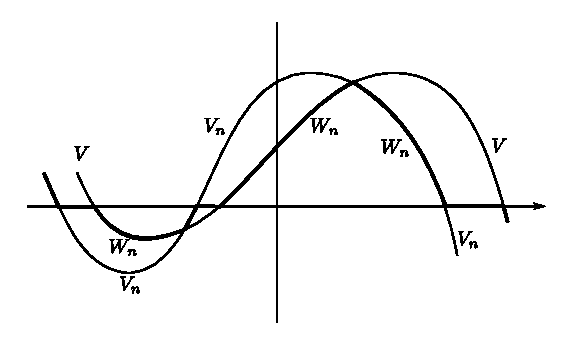
\includegraphics{vol65-figures/fig65-chap2.2.eps}}
\caption{}
\end{figure}

Then\pageoriginale  
\begin{align}
& w_n \text{ has a compact support in }\Omega, \tag{2.62}\label{c4:eq2.62}\\
& || w_n ||_{L^\infty(\Omega)} \leq ||v||_{L^\infty(\Omega)} \tag{2.63}\label{c4:eq2.63}
\end{align}
and it follows from Chap.~\ref{chap2}, Corollary~\ref{c2:cor2.1}, that 
\begin{equation}
\lim_{n \to \infty} w_n = v \text{ strongly in }V. \tag{2.64}\label{c4:eq2.64}
\end{equation}
\end{proof}

From \eqref{c4:eq2.63} and \eqref{c4:eq2.64} we obtain that $\lim\limits_{n \to \infty} w_n = v$ for the \textit{weak} * \textit{topology} of $L^\infty(\Omega)$.

Thus we have proved that 
$$
\mathscr{U}  = \{v \in L^\infty (\Omega) \cap V : v \text{ has compact support in }\Omega\}
$$
is dense in $L^\infty (\Omega) \cap V$ for the topology given in the statement of the Lemma. 

Let $v \in \mathscr{U}$ and $(\rho_n)_n$ be a mollifying sequence 
(see Chap.~\ref{chap2}, Lemma\break\ref{c4:lem2.4}). Define $\tilde{v}_n$ by 
\begin{equation}
\tilde{v} (x) = 
\begin{cases}
v(x) & \text{ if } x \in \Omega, \\
{}\\
0 & \text{ if } x \not\in \Omega,
\end{cases}
\end{equation}
\begin{align}
& \tilde{v}_n = \rho_n * \tilde{v}, \tag{2.66}\label{c4:eq2.66}\\
& \text{ then } \tilde{v}_n  \in \mathscr{D} (\mathbb{R}^N), \lim_{n \to \infty} \tilde{v}_n = \tilde{v} \text{ strongly in } H^1(\mathbb{R}^N), \tag{2.67}\label{c4:eq2.67}\\
& \tilde{v}_n \text{ has a compact support in }\Omega \text{ for } n \text{ large enough}. \tag{2.68}\label{c4:eq2.68}
\end{align}

Let $v_n = \tilde{v}_n |_\Omega$ then for $n$ large enough $v_n \in \mathscr{D}(\Omega)$ and $\lim \limits_{n \to \infty} v_n = v$ \textit{strongly} on $V$.

Since $|| \tilde{v} ||_{L^\infty(\mathbb{R}^N)} = || v ||_{L^\infty(\Omega)}$ it follows from \eqref{c4:eq2.66} that 
\begin{equation}
|v_n(x) | \leq \int_{\mathbb{R}^N} \rho_n (x-y) | \tilde{v}(y) |dy \leq || v 
||_{L^\infty(\Omega)} \tag{2.69}\label{c4:eq2.69}
\end{equation}
From\pageoriginale  this it follows that 
\begin{equation}
|| v_n ||_{L^\infty(\Omega)} \leq || v ||_{L^\infty(\Omega)} \tag{2.70}\label{c4:eq2.70}
\end{equation}
Summarising the above information we have proved that $\forall v \in 
L^{\infty}(\Omega) \cap V$, there exists a sequence $(v_n)_n$, $v_n \in 
\mathscr{D} (\Omega)\, \forall n$, such that 
\begin{align}
& \lim_{n \to \infty} v_n = v \text{ strongly in } V, \tag{2.71}\label{c4:eq2.71}\\
& || v_n ||_{L^{\infty}(\Omega)} \leq || v ||_{L^\infty(\Omega)}\, \forall n. \tag{2.72}\label{c4:eq2.72}
\end{align}
Hence from \eqref{c4:eq2.71} and \eqref{c4:eq2.72} we obtain that $v_n \to v$ in $L^{\infty}(\Omega)$ \textit{weak} *. This completes the proof of the Lemma.

\begin{theorem}\label{c4:thm2.2}%theo 2.2
Under the above hypothesis on $V$, $a(\cdot , \cdot)$, $L(\cdot)$,
$\phi(\cdot)$,  problems $(\pi)$ and $(P)$ are equivalent. 
\end{theorem}

\begin{proof}
We have already proved that $(\pi)$ implies $(P)$. We need only to
prove that $(P)$ implies $(\pi)$. 

From the definition of $(P)$ we have 
\begin{equation}
\begin{cases}
a(u, v) + < \phi (u), v> = L(v) ~~ \forall v \in V,\\
&\\
u \in V, \phi (u) \in H^{-1}(\Omega) \cap L^1(\Omega).
\end{cases}
\tag{2.73}\label{c4:eq2.73}
\end{equation}
It follows from \eqref{c4:eq2.73} that 
\begin{equation*}
a(u, v) + \int_\Omega \phi (u)v dx = L(v) ~~ \forall v \in \mathscr{D}(\Omega). \tag{2.74}\label{c4:eq2.74}
\end{equation*}
\end{proof}

If $v \in V \cap L^\infty (\Omega)$ we know from Lemma \ref{c4:lem2.5}
that there exists a sequence $(v_n)_n$, $v_n \in \mathscr{D}(\Omega)$,
such that  
\begin{align}
& \lim_{n \to \infty} v_n = v \text{ strongly in } V,
  \tag{2.75}\label{c4:eq2.75}\\ 
& \lim_{n \to \infty} v_n = v \text{ in } L^\infty(\Omega) \text{ weak
  } *. \tag{2.76}\label{c4:eq2.76} 
\end{align}
Since\pageoriginale  $v_n \in \mathscr{D}(\Omega)$ we have, from
(\ref{c4:eq2.74}),  
\begin{equation}
a(u, v_n) + \int_\Omega \phi(u) v_n dx = L(v_n). \tag{2.77}\label{c4:eq2.77}
\end{equation}
It follows from \eqref{c4:eq2.77} that $\lim\limits_{n \to \infty} a (u, v_n) = a(u, v)$, $\lim\limits_{n \to \infty} L (v_n) = L(v)$ and, since $\phi (u) \in L^1(\Omega)$, \eqref{c4:eq2.76} implies that 
$$
\lim_{n \to \infty} \int_\Omega \phi(u)v_n dx = \int_\Omega \phi (u) v dx.
$$
Thus taking the limit in \eqref{c4:eq2.77}, we obtain 
$$
a(u, v) + \int _\Omega \phi(u) v dx = L(v) ~ \forall v \in V \cap L^\infty (\Omega).
$$
Therefore $(P)$ implies \eqref{c4:eq2.47} which implies in turn $(\pi)$. This completes the proof of the Theorem.

\begin{exercise}\label{c4:exer2.2}%2.2
Find in $\mathbb{R}^2$, a function $v$ such that $v \notin H^{-1}(\Omega) \cap L^1(\Omega)$, $v \not \in L^p(\Omega)\, \forall_p > 1$, where $\Omega$ is some bounded open set in $\mathbb{R}^2$.
\end{exercise}

\begin{exercise}\label{c4:exer2.3}%2.3
Prove that if $u \geq 0$ a.e. then $\phi (u) v \in L^1(\Omega)$  $\forall v \in V$, where $u$ is the solution of the problem $(P)$.
\end{exercise}

\subsection{Some comments on the continuous problem}\label{c4:ss2.4} 

We have studied $(P)$ and $(\pi)$ with rather weak hypotheses, namely
$\phi \in C^0(\mathbb{R})$ and nondecreasing, and $f \in V^*$. The
proof we have given for the equivalence between $(P)$ and $(\pi)$ can
be made shorter using more sophisticated tools of Convex Analysis and
from the theory of Monotone Operators (see LIONS [\ref{k67:e1}] and the
bibliography therein). However our proof is very elementary and some
of the lemmas we have obtained will be useful in the numerical
analysis of the problem $(P)$. \textit{Regularity results} for
problems little more complicated that $(P)$ and $(\pi)$ are given in
BREZIS-CRANDALL-PAZY [\ref{k17:e1}] ; in particular for $f \in L^2(\Omega)$ and
with convenient smoothness assumptions for $A$, the
$H^2(\Omega)$-regularity of $u$ is proved.  

\subsection{Finite element approximation of $(\pi)$ and $(P)$}\label{c4:ss2.5}

\subsubsection{Definition of the approximate
  problem}\label{c4:sss2.5.1}\pageoriginale   

Let $\Omega$ be a bounded \textit{polygonal} domain of $\mathbb{R}^2$ and $\mathscr{C}_h$ be a triangulation of $\Omega$ satisfying \eqref{c4:eq2.21}- \eqref{c4:eq2.23} of Chap. 2. We approximate $V$ by 
$$
V_h = \{v_h \in C^0 (\overline{\Omega}) : v_h |_\Gamma = 0, v_h |_T \in P_1\, \forall T \in \mathscr{C}_h\}.
$$
Then it is natural to approximate $(P)$ and $(\pi)$ respectively by 
\begin{align*}
& \begin{cases}
a (u_h, v_h) + \int_\Omega \phi (v_h) v_h dx = L(v_h)\, \forall v_h \in V_h,\\
&\\
u_h \in V_h
\end{cases} \tag{$P^*_h$}\\
\text{ and }\\
& \begin{cases}
a(u_h, v_h - u_h) +  j(v_h) - j(u_h) \geq L(v_h - u_h)\, \forall v_h \in V_h,\\
&\\
u_h \in V_h
\end{cases} \tag{$\pi^*_h$}
\end{align*}
with
$$
j(v_h) = \int_\Omega \phi (v_h) dx.
$$
Obviously $(P^*_h)$ and $(\pi^*_h)$ are equivalent. From a
computational point of view we cannot use in general $(P^*_h)$ and
$(\pi^*_h)$ directly since they involve the computation of integrals
which cannot be done exactly. For this reason we shall have to modify
$(\pi^*_h)$ and $(P^*_h)$ using somewhere some \textit{numerical
  integration procedures.} Actually we shall have to approximate
$a(\cdot, \cdot)$, $L(\cdot)$ and $j(\cdot)$. Since the approximation
of $a(\cdot, \cdot)$ and $L(\cdot)$ is studied in CIARLET [1, Chap. 8]
we shall assume that we still work with $a(\cdot, \cdot)$ and
$L(\cdot)$ but we shall approximate $j(\cdot)$. 

To approximate $j(\cdot)$ we shall use the \textit{two dimensional 
trapezoidal method}. Hence using the notation of Figure~2.3 below we approximate $j(\cdot)$ by 
\begin{equation}
j_h(v_h) = \sum_{T \in \mathscr{C}_h} \frac{meas \cdot (T)}{3} \sum^3_{i=1} \Phi (v_h(M_{iT}))\, \forall v_h \in V_h. \tag{2.78}\label{c4:eq2.78}
\end{equation}

\begin{figure}[H]
\centering{\includegraphics{vol65-figures/fig65-chap2.3.eps}}
\caption{}
\end{figure}

Actually\pageoriginale  $j_h(v_h)$ may be viewed as the exact integral of some piecewise constant functions.

Using the notation of Chap.~\ref{chap2}, Sec.~\ref{c4:ss2.5}, assume 
that the set $\sum_h$ of the nodes of $\mathscr{C}_h$ has been ordered 
by $i=1, 2, \ldots, N_h$ where $n_h = Card( \sum_h)$. Let $M_i \in 
\sum_h$. We define a domain $\Omega_i$ by joining, as in 
Figure~2.4, the centroids of the triangles, admitting $M_i$ as a common vertex, to the midpoint of the edges admitting $M_i$ as a common extremity (if $M_i$ is a boundary point the modification of 
Figure~2.4 is trivial to do).

\begin{figure}[H]
\centering{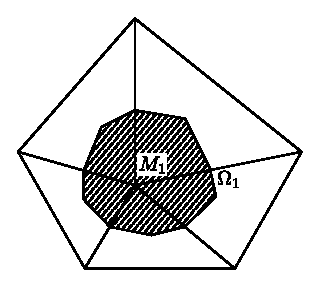
\includegraphics{vol65-figures/fig65-chap2.4_1.eps}}
\caption{}
\end{figure} 

Let us define the space of piecewise functions :
\begin{equation}
L_h = \{\mu_h : \mu_h = \sum^{N_h}{i=1} \mu_i \chi_i, \mu_i \in
\mathbb{R}, i = 1, 2, \ldots, N_h\}, \tag{2.79}\label{c4:eq2.79} 
\end{equation}
where\pageoriginale  $\chi_i$ is the characteristic function of $\Omega_i$.

We then define $q_h : C^0 (\overline{\Omega}) \cap H^1_0 (\Omega) \to L_n$ by 
\begin{equation}
q_h v = \sum^{N_h}_{i=1}v(M_i) \chi_i. \tag{2.80}\label{c4:eq2.80}
\end{equation}
Then it follows from \eqref{c4:eq2.79} and \eqref{c4:eq2.80} that
\begin{equation}
j_h (v_h) = \int_\Omega \Phi (q_h v_h)dx\, \forall v_h \in V_h. \tag{2.81}\label{c4:eq2.81}
\end{equation}
We also have 
\begin{equation}
j_h(v_h) = j(q_h v_h)\, \forall v_h \in V_h. \tag{2.82}\label{c4:eq2.82}
\end{equation}
Then we approximate $(P)$ and $(\pi)$ by 
\begin{align*}
& \begin{cases}
a(u_h, v_h) + \int_\Omega \phi (q_h u_h) q_h v_h dx = L(v_h)\, \forall v_h \in V_h,\\
&\\
u_h \in V_h
\end{cases} \tag{$P_h$}\\
and\\
& \begin{cases}
a(u_h, v_h-u_h) + j_h(v_h) -j_h(u_h) \geq L(v_h-u_h)\, \forall v_h \in V_h,\\
&\\
u_h \in V_h.
\end{cases} \tag{$ \pi_h $}
\end{align*}
Then

\begin{theorem}\label{c4:thm2.3}%the 2.3
Problem $(P_h)$ and $(\pi_h)$ are equivalent and have a unique solution.
\end{theorem}

\begin{exercise}\label{c4:exer2.4}%exe 2.4
Prove Theorem~\ref{c4:thm2.3}.
\end{exercise}

\subsubsection{Convergence of the approximate solutions}\label{c4:sss2.5.2}

\begin{theorem}\label{c4:thm2.4}%the 2.4
If as $h \to 0$ the angles of $\mathscr{C}_h$ are uniformly bounded below by $\theta_0 > 0$ then
$$
\lim_{h \to 0} ||u_h - u ||_V = 0,
$$
where $u$ and $u_h$ are respectively the solutions of $(P)$ and $(P_h)$.
\end{theorem}

\begin{proof}%pro
Since\pageoriginale  $j(\cdot)$ is {\em not continuous} on $V$, the result of Chap. 1, 
Sec. 6 on the approximation of EVI of the second kind cannot be applied 
directly. However the proof of the convergence follows the same lines 
as in Theorem~\ref{c1:thm6.2} of Chap.~\ref{chap1}.
\end{proof}
\begin{enumerate}[(1)]
\item {\bf A priori estimates for $u_h$.} Taking $v_h = 0$ in $(\pi_h)$ we obtain 
\begin{align}
& ||u_h||_V \leq \frac{|| f ||}{\alpha}. \tag{2.83}\label{c4:eq2.83}\\
& 0 \leq \int_\Omega \Phi (q_h u_h) dx \leq \frac{||f||^2} {\alpha}. \tag{2.84}\label{c4:eq2.84}
\end{align}

\item {\bf Weak convergence of $u_h$.} It follows from \eqref{c4:eq2.83} and from the compactness of the injection of $V$ in $L^2(\Omega)$, that we can extract from $(u_h)_h$ a subsequence, still denoted by $(u_h)_h$, such that 
\begin{align}
u_h & \to u^* \text{ weakly in }V, \tag{2.85}\label{c4:eq2.85}\\
u_h & \to u^* \text{ strongly in } L^2 (\Omega), \tag{2.86}\label{c4:eq2.86}\\
u_h & \to u^* \text{ a.e. in }\Omega. \tag{2.87}\label{c4:eq2.87}
\end{align}
\end{enumerate}

Admitting for the moment the following inequality
\begin{equation}
||q_h v_h - v_h||_{L^p(\Omega)} \leq \frac{2h}{3} ||\nabla v||_{L^p(\Omega) \times L^p(\Omega)}\, \forall v_h \in V_h,\, \forall p \text{ with } 1 \leq p \leq \infty, \tag{2.88}\label{c4:eq2.88}
\end{equation}
it follows from \eqref{c4:eq2.83} and \eqref{c4:eq2.86} that 
\begin{equation}
q_h u_h \to u^* \text{ strongly in }L^2(\Omega). \tag{2.89}\label{c4:eq2.89}
\end{equation}

Then, modulo another extraction of a subsequence, we have
\begin{equation}
q_h u_h \to u^* \text{ a.e. in }\Omega, \tag{2.90}\label{c4:eq2.90}
\end{equation}
from which it follows that 
\begin{equation}
\Phi (q_h u_h) \to \Phi (u^*) \text{ a.e. in } \Omega. \tag{2.91}\label{c4:eq2.91}
\end{equation}

Then\pageoriginale  taking $v \in \mathscr{D}(\Omega)$, it follows
from CIARLET [\ref{k31:e1}], [\ref{k31:e2}], STRA\-NG-FIX [\ref{k85:e1}]
that under the assumptions on 
$\mathscr{C}_h$ of the statement of the Theorem we have  
\begin{align}
||r_h v-v||_{W^{1, \infty}(\Omega)} & \leq Ch ||v||_{W^{2, \infty}(\Omega)}\, \forall v \in \mathscr{D}(\Omega), \tag{2.92}\label{c4:eq2.92}\\
||r_h v-v||_{L^{\infty}(\Omega)} & \leq Ch^2 ||v||_{W^{2, \infty}(\Omega)}\, \forall v \in \mathscr{D}(\Omega), \tag{2.93}\label{c4:eq2.93}
\end{align}
where $C$ is a constant independent of $v$ and $h$ and where $r_h$ is the usual linear interpolation operator over $\mathscr{C}_h$. Moreover \eqref{c4:eq2.88} with $p = + \infty$, \eqref{c4:eq2.92} and \eqref{c4:eq2.93} imply that 
\begin{equation}
\lim_{h \to 0} ||q_h r_h v - v||_{L^{\infty}(\Omega)} = 0\, \forall v \in 
\mathscr{D}(\Omega). \tag{2.94}\label{c4:eq2.94}
\end{equation}
Taking $v_h = r_h v$ in $(\pi_h)$ we obtain 
\begin{align*}
a(u_h, u_h) & + \int_\Omega \Phi (q_h u_h) dx \leq a(u_h, r_h v)\\ 
& +\int_\Omega \Phi  
(q_h r_h v) dx - L(r_h v-u_h)\, \forall v \in \mathscr{D}
(\Omega). \tag{2.95}\label{c4:eq2.95} 
\end{align*}
From \eqref{c4:eq2.85}, \eqref{c4:eq2.89} and Lemma~\ref{c4:lem2.1} we have
$$
a(u^*, u^*) + \int_\Omega \Phi (u^*) dx \leq\lim \inf (a(u_h, u_h) 
+ \int_\Omega \Phi (q_h u_h)dx).
$$
Moreover 
$$
\lim_{h \to 0} \int_\Omega \Phi(q_h r_h v)dx = \int_\Omega \Phi(v)dx = j(v) 
\forall v \in \mathscr{D} (\Omega).
$$
Then in the limit in \eqref{c4:eq2.95} we obtain
\begin{equation}
a(u^*, u^*) + j(u^*) \leq a(u^*, v) +j(v)-L(v-u^*)\, \forall v \in 
\mathscr{D}(\Omega). \tag{2.96}\label{c4:eq2.96}
\end{equation}
From Fatou's lemma applied to \eqref{c4:eq2.84} and \eqref{c4:eq2.91} we obtain 
\begin{equation}
\Phi (u^*) \in L^1(\Omega). \tag{2.97}\label{c4:eq2.97}
\end{equation}
Then it follows from \eqref{c4:eq2.96} and \eqref{c4:eq2.97} that $u^*$ satisfies 
\begin{equation}
a(u^*, v - u^*) + j(v) - j(u^*) \leq L(v-u^*)\, \forall v \in 
\mathscr{D}(\Omega), u^* \in V, \phi (u^*) \in L^1(\Omega). \tag{2.98}\label{c4:eq2.98}
\end{equation}

We now\pageoriginale  take $v \in V \cap L^\infty (\Omega)$, it follows from 
Lemma~\ref{c4:lem2.5} that there exists a sequence $(v_n)_n$, $v_n \in \mathscr{D}(\Omega)$ such that 
\begin{align}
\lim_{n \to \infty} v_n & = v \text{ strongly in }V, \tag{2.99}\label{c4:eq2.99}\\
\lim_{n \to \infty} v_n & = v \text{ in }L^\infty (\Omega) \text{ weak }^*. \tag{2.100}\label{c4:eq2.100}
\end{align}
We have from \eqref{c4:eq2.98} that 
\begin{equation}
a(u^*, v_n-u^*) + j(u_n) - j(u^*) \geq L(v_n - u^*)\, \forall n, u^* \in V, 
\Phi (u^*) \in L^1(\Omega). \tag{2.101}\label{c4:eq2.101}
\end{equation}
We obviously have from \eqref{c4:eq2.99}
\begin{align*}
& \lim_{n \to \infty} a(u^*, v_n - u^*) = a(u^*, v-u^*),\\
& \lim_{n \to \infty} L(v_n - u^*) = L(v-u).
\end{align*}

Since $v_n \to v$ in the weak * topology of $L^\infty(\Omega)$ we have a constant $C$ such that 
\begin{equation}
||v_n||_{L^{\infty}(\Omega)} \leq C\, \forall n. \tag{2.102}\label{c4:eq2.102}
\end{equation}
Moreover, for some subsequence, \eqref{c4:eq2.99} implies that 
\begin{equation}
\lim_{n \to \infty} v_n = v \text{ a.e. in } \Omega. \tag{2.103}\label{c4:eq2.103}
\end{equation}
From \eqref{c4:eq2.103} we obtain that 
$$
\Phi (v_n) \to \Phi (v) \text{ a.e. in } \Omega.
$$
From \eqref{c4:eq2.102} and \eqref{c4:eq2.103} one can easily see that the Lebesgue 
dominated convergence theorem can be applied to $(Phi(u_n))_n$. Hence we obtain 
$$
\lim_{n \to \infty} j (v_n) = \lim_{n \to \infty} \int_\Omega 
\Phi (v_n) dx = \int_\Omega \Phi (v)dx = j(v).
$$
Therefore\pageoriginale  taking the limit in \eqref{c4:eq2.101} we obtain
\begin{equation}
\begin{cases}
a(u^*, v - u^*) + j(v) - j(u^*) \geq L(v - u)^*)\, \forall v \in V \cap L^\infty (\Omega),\\
&\\
u^* \in V, \Phi(u^*) \in L^1(\Omega).
\end{cases} \tag{2.104}\label{c4:eq2.104}
\end{equation}

Since from Lemma~\ref{c4:lem2.2} we know that \eqref{c4:eq2.104} is
equivalent to $(\pi)$ we have proved that $u^* = u$ where $u$ is the
solution of $(\pi)$. From the uniqueness of the solution of $(\pi)$ it
follows that the whole sequence $(u_h)_h$ converges to $u$. 
\begin{enumerate}
\item[(3)] {\bf Strong convergence of $(u_h)_h$} :  From the
  $V$-ellipticity of $a(\cdot, \cdot)$ and from the variational
  inequality satisfied by $u_h$ we obtain  
\begin{equation}
\begin{cases}
\alpha ||u_h - u||^2 + j_h(u_h) \leq a(u_h - u, u_h - u) + j_h(u_h)\\
\hspace{3cm}\leq -a(u_h, u) + a(u, u) + a(u_h, u_h)\\ 
-a(u, u_h) + j_h(u_h) \leq -a(u_h, u) + a(u, u) + a(u_h, r_h v)\\ 
\hspace{3cm} + j_h(r_h v) - L(r_h v - u_h)\\ 
-a(u, u_h) ~~\, \forall v \in \mathscr{D}(\Omega).
\end{cases}\tag{2.105}\label{c4:eq2.105}
\end{equation}
\end{enumerate}
Using the various convergence results of Part (2) we obtain from \eqref{c4:eq2.105} that 
\begin{equation}
\begin{cases}
j(u) & \leq \lim \inf j_h(u_h) \leq \lim \inf (\alpha ||u_h - u||^2_V
+ j_h (u_h))\\ 
& \leq \lim \sup (\alpha ||u_h - u||^2 + j_h(u_h))\\ 
& \qquad \leq a(u, v - u) + j(v) - L(v - u) ~~\, \forall v \in \mathscr{D}(\Omega).
\end{cases}\tag{2.106}\label{c4:eq2.106}
\end{equation}
Using as in Part (2) the density of $\mathscr{D}(\Omega)$ in $L^\infty(\Omega) \cap V$ (for the strong topology of $V$ and the weak * topology of $L^\infty(\Omega))$, we obtain that \eqref{c4:eq2.106} also holds for all $v \in V \cap L^\infty(\Omega)$. Then 
\begin{equation}
\begin{cases}
j(u) & \leq \lim \inf j_h(u_h) \leq \lim \inf (\alpha ||u_h - u||^2_V
+ j_h(u_h)) \\ 
& \leq \lim \sup (\alpha ||u_h - u||^2_V + j_h(u_h))\\ 
& \qquad \leq a(u, \tau_n v - u) + j
(\tau_n v) - L(\tau_n v - v) ~~\forall v \in V.
\end{cases}\tag{2.107}\label{c4:eq2.107}
\end{equation}
Using the properties of $\tau_n v$, it follows then from \eqref{c4:eq2.107}, by taking the limit as $n \to \infty$, that \eqref{c4:eq2.106} also holds for all $v \in V$. Hence by taking $v=u$ we obtain 
\begin{equation*}
\begin{cases}
j(u) & \leq \lim \inf j_h(u_h) \leq \lim \inf (\alpha ||u_h - u||^2 + j_h(u_h))\\
& \leq \lim \sup (\alpha ||u_h - u||^2 +j_h(u_h)) \leq j(u),
\end{cases}
\end{equation*}
which\pageoriginale  implies 
\begin{align*}
& \lim_{h \to 0} j_h (u_h) = j(u),\\
& \lim_{h \to 0} ||u_h - u||_V = 0. 
\end{align*}
This proves the Theorem modulo the proof of \eqref{c4:eq2.88}. 
We now prove \eqref{c4:eq2.88}.

\begin{lemma}\label{c4:lem2.6}%lem 2.6
We have 
$$\forall p, 1 \leq p \leq \infty, ||q_h v_h - v_h||_{L^p(\Omega)}
\leq \dfrac{2}{3}h ||\nabla v_h||_{L^p(\Omega) \times L^p(\Omega)}$$  
where $q_h$, $v_h$ are as before.
\end{lemma}

\begin{proof}%pro 
We use the notation of Sec.~\ref{c4:sss2.5.1}
\end{proof}

\begin{figure}[H]
\centering{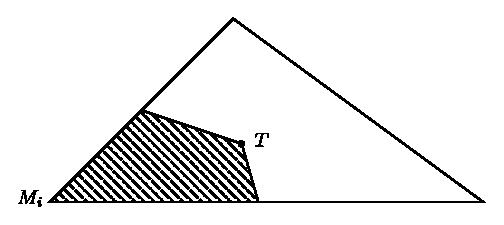
\includegraphics{vol65-figures/fig65-chap2.5_1.eps}}
\caption{}\label{c4:fig2.5}
\end{figure} 

We have (see Figure \ref{c4:fig2.5})
\begin{equation}
|v_h (M) - q_h v_h(M)| = |v_h(M_i) - v_h(M)| \ \forall M \in \Omega_i 
\cap T. \tag{2.108}\label{c4:eq2.108}
\end{equation}
But since $v_h|_T \in P_1$ we have
$$
v_h(M) = v_h (M_i)+ \overrightarrow{M_i M} \cdot \nabla v_h \quad 
\forall M \in \Omega_i \cap T,
$$
from which it follows, combined with \eqref{c4:eq2.108}, that 
$$
|q_h v_h(M) - v_h(M)| \leq |\overrightarrow{M_i M|} |\nabla v_h| \ \forall M 
\in \Omega_i \cap T.
$$

But\pageoriginale  from the definition of $h$ we have $|\overrightarrow{M_i M}|\leq \dfrac{2}{3}h \ \forall T$ so that we finally have $|q_h v_h (x) - v_h(x)| \leq \dfrac{2}{3} h |\nabla v_h(x)|$ a.e. in $\Omega$, $\forall v_h \in V_h$. This implies 
$$
||q_h v_h - v_h ||_{L^p(\Omega)} \leq \frac{2}{3} h ||\nabla v_h||_{L^p(\Omega) \times L^p(\Omega)}.
$$
This proves the lemma.

\begin{remark}\label{c4:rem2.4}%rem 2.4
We have not considered the problem of error estimates. This problem
will be discussed in GLOWINSKI [\ref{k51:e4}]. 
\end{remark}

\begin{remark}\label{c4:rem2.5}%rem 2.5
The numerical analysis of problem like $(P)$ but with much stronger
hypotheses on $a(\cdot, \cdot)$, $\phi$, $f$ is considered in CIARLET
- SCHULTZ - VARGA [\ref{k33:e1}]. 
\end{remark}

\subsection{Iterative methods for solving the discrete problem}\label{c4:ss2.6}

\subsubsection{Introduction}\label{c4:sss2.6.1} 

In this section we briefly describe some \textit{iterative methods} 
which may be useful for computing the solution of $(P_h)$ (and 
$(\pi_h)$). Actually most of these methods can be extended to other 
non-linear problems. Many of the methods to be described here can be 
found in ORTEGA-\break RHEINBOLDT [\ref{k76:e1}]. A method based on \textit{duality} 
techniques will be described in Chap.~\ref{chap5}.

\subsubsection{Formulation of the discrete problem}\label{c4:sss2.6.2}

Here we are using the notation of the continuous problem. Taking as
unknowns the values of $u_h$ at the interior nodes of $\mathscr{C}_h$,
the problem $(P_h)$ reduces to the finite dimensional non-linear
problem  
\begin{equation}
\A\limits_\sim \uu\limits_\sim + \D\limits_\sim \phi (\uu\limits_\sim) = 
\f\limits_\sim,\tag{2.109}\label{c4:eq2.109}
\end{equation}
where $\A\limits_\sim$ is a $N \times N$ positive definite matrix, $\D\limits_\sim$ is a diagonal matrix with positive diagonal elements $d_i'$s and where $\uu\limits_\sim = \{u_1, \ldots, u_N\} \in \mathbb{R}^N$, $\f\limits_\sim \in \mathbb{R}^N$, $\phi (\uu\limits_\sim) \in \mathbb{R}^N$ with $(\phi(\uu\limits_\sim))_i = \phi (u_i)$. Clearly from the properties of $\A\limits_\sim$, $\D\limits_\sim$, $\phi$, $\f\limits_\sim$ we can see that the problem \eqref{c4:eq2.109} has a unique solution. 

\subsubsection{Gradient Methods}\label{c4:sss2.6.3} 

The basic\pageoriginale  algorithm with constant step (see CEA [1]) is given by
\begin{align}
& \uu\limits_\sim ^{0} \in \mathbb{R}^N \text{ given },
  \tag{2.110}\label{c4:eq2.110}\\ 
& \uu\limits_\sim^{n+1} = \uu\limits_\sim^n- \rho {\s\limits_\sim}^{-1}
  (\A\limits_\sim {\uu\limits_\sim}^n + \D\limits_\sim \phi
  ({\uu\limits_\sim}^n) - \f\limits_\sim ), \rho >
  0. \tag{2.111}\label{c4:eq2.111} 
\end{align}

In \eqref{c4:eq2.111}, $\s\limits_\sim$ is a \textit{symmetric,
  positive definite matrix}: a canonical choice is $\s\limits_\sim$ =
\textit{Identity}. But in most problems it will give a \textit{slow
  speed of convergence}. If $A$ is symmetric, the natural choice is
$\s\limits_\sim = \A\limits_\sim$ and, if $\A\limits_\sim \neq
\A\limits_\sim^*$, we can take $\s\limits_\sim =
\dfrac{\A\limits_\sim+ \A\limits_\sim^*}{2}$. 

For the convergence of ${\uu\limits_\sim}^n$ to $\uu\limits_\sim$ (where
$\uu\limits_\sim$ is the solution of \eqref{c4:eq2.109}) it is
sufficient to have $\phi$ smooth enough (for example, $\phi$ locally
Lipschitz continuous). Then $\lim\limits_{n \to \infty}
{\uu\limits_\sim}^n = \uu\limits_\sim$ if $\rho$ is sufficiently
small. Obviously the closer ${\uu\limits_\sim}^0$ is to
$\uu\limits_\sim$, the faster is the convergence. 

\begin{remark}\label{c4:rem2.6}%rem 2.6
If $\A\limits_\sim = \A \limits_\sim ^*$, then $\A\limits_\sim \V
\limits_\sim  +\D \limits_\sim \phi (\V\limits_\sim)-\f \limits_\sim$
is the gradient at $\V\limits_\sim$ of the functional
$j(\V\limits_\sim) = \dfrac{1}{2} (A \V\limits_\sim, \V\limits_\sim) +
\sum \limits^{N}_{i=1} d_i \Phi (v_i) -(\f\limits_\sim,
\V\limits_\sim)$, where $(\cdot, \cdot)$ denotes the usual inner
product of $\mathbb{R}^N$ and $\Phi(t) = \int^t_0 \phi (\tau)d \tau$. 
\end{remark}

\begin{remark}\label{c4:rem2.7}%rem 2.7
In each specific case $\rho$ has to be determined ; this can be done theoretically, experimentally or by using an automatic adjustment procedure which will not be described here.
\end{remark}

\begin{remark}\label{c4:rem2.8}%rem 2.8
Let us define ${\g\limits_\sim}^n$ by
$$
{\g\limits_\sim}^n = \A\limits_\sim {\uu\limits_\sim}^n + \D\limits_\sim \phi 
({\uu\limits_\sim}^n) - \f\limits_\sim.
$$
Instead of using a constant parameter $\rho$ we can use a family $(\rho_n)_n$ of positive parameters in 
\eqref{c4:eq2.111}. Therefore \eqref{c4:eq2.111} can be written as 
\begin{equation}
{\uu\limits_\sim}^{n+1}= {\uu\limits_\sim}^n -\rho_n
\s\limits_\sim^{-1}{\g\limits_\sim}^n.\tag{2.112}\label{c4:eq2.112}
\end{equation}
Suppose $\A\limits_\sim = \A\limits_\sim^*$, then if we use \eqref{c4:eq2.110}, 
\eqref{c4:eq2.112} with $\rho_n$ defined by 
\begin{equation}
\begin{cases}
J({\uu\limits_\sim}^n- \rho_n \s\limits_\sim^{-1}{\g\limits_\sim}^n)
\leq J({\uu\limits_\sim}^n - 
\rho \s\limits_\sim^{-1}{\g\limits_\sim}^n) ~~ \forall \rho \in \mathbb{R},\\
&\\
\rho_n \in \mathbb{R},
\end{cases} \tag{2.113}\label{c4:eq2.113}
\end{equation}\pageoriginale 
the resulting algorithm is, for obvious reasons, called
\textit{steepest descent method}. This algorithm is convergent for
$\phi \in C^0(\mathbb{R})$. We observe that at each iteration the
determination of $\rho_n$ requires the solution of a one-dimensional
problem; for the solution of such one dimensional problems see
HOUSEHOLDER [\ref{k57:e1}], POLAK [\ref{k77:e1}], BRENT [\ref{k13:e1}]. 
\end{remark}

\begin{remark}\label{c4:rem2.9}%rem 2.9
At each iteration of \eqref{c4:eq2.110}, \eqref{c4:eq2.111} or
\eqref{c4:eq2.110}, \eqref{c4:eq2.112} we have to solve a linear
system related to $\s\limits_\sim$. Since $\s\limits_\sim$ is
symmetric and positive definite this system can be solved using
Cholesky method, provided the $\s\limits_\sim = \el\limits_\sim 
\el\limits_\sim^*$ factorization has been done. From a practical
point of view it is obvious that the factorization of $\s\limits_\sim$
will be made in the beginning once for all. Then at each iteration we
just have to solve two triangular systems which is a trivial
operation. 
\end{remark}

\subsubsection{Newton's method}\label{c4:sss2.6.4} 
The Newton's algorithm is given by (for sufficient conditions of
convergence, see ORTEGA-RHEINBOLDT [\ref{k76:e1}]) : 
\begin{align}
& {\uu\limits_\sim}^0 \in \mathbb{R}^N  \text{ given },
  \tag{2.114}\label{c4:eq2.114}\\ 
& {\uu\limits_\sim}^{n+1} = (\A\limits_\sim+ \D\limits_\sim \phi'
  ({\uu\limits_\sim}^n))^{-1} (\D\limits_\sim \phi' ({\uu\limits_\sim}^n)
  {\uu\limits_\sim}^n -\D\limits_\sim \phi ({\uu\limits_\sim}^n) +
  \f\limits_\sim) \tag{2.115}\label{c4:eq2.115} 
\end{align}
where $\phi'(\V\limits_\sim)$ denotes the \textit{diagonal matrix}
\begin{equation*}
\phi'(\V \limits_\sim  ) =
\begin{pmatrix}
\phi'(v_1) \ddots & 0\\
& \ddots  &\\
0 & \phi'(v_n)
\end{pmatrix}
\end{equation*}

Since $\phi$ is nondecreasing, $\phi' \geq 0$. This implies that $\A \limits_\sim+\D \limits_\sim \phi' (\V \limits_\sim)$ is positive definite $\forall \V \limits_\sim \in \mathbb{R}^N$.

\begin{remark}\label{c4:rem2.10}%rem 2.10
At each iteration we have to solve a linear system. Since the matrix
$\A\limits_\sim + \D \limits_\sim \phi'({\uu \limits_\sim}^n)$ depends
on $n$, this method may not be convenient for large $N$. 
\end{remark}

\begin{remark}\label{c4:rem2.11}%rem 2.11
The choice of ${\uu\limits_\sim}^0$ is very important when using
Newton's method. 
\end{remark}

\subsubsection{Relaxation and over-relaxation
  methods}\label{c4:sss2.6.5} 

We use\pageoriginale  the following notation :
\begin{align*}
\A\limits_\sim & = (a_{ij})_{1 \leq i, j \leq N},\\
\f \limits_\sim & = \{f_1, f_2, \ldots, f_N\}.
\end{align*}

Since $\A \limits_\sim$ is \textit{positive definite} we have $a_{ii}
> 0\, \forall i=1, 2, \ldots, N$. Here we will describe three
algorithms: 

\begin{algorithm}\label{c4:alg1} %algorithm 1
\begin{equation}
{\uu \limits_\sim}^0 \in \mathbb{R}^N \text{ given },
\tag{2.116}\label{c4:eq2.116} 
\end{equation}
then given ${\uu \limits_\sim}^n$, we compute ${\uu
  \limits_\sim}^{n+1}$, component by component, using 
\begin{align}
& a_{ii}u_i^{-n+1} + d_i \phi (u_i^{-n+1}) = f_i - \sum_{j<i} a_{ij} u_j^{n+1} - \sum_{j  > i} a_{ij} u^n_j, \tag{2.117}\label{c4:eq2.117}\\
& u_i^{n+1} = u^n_i + \omega (u_i^{-n+1}-u^n_i), i=1, 2, \ldots, N. \tag{2.118}\label{c4:eq2.118}
\end{align}
\end{algorithm}

Since $a_{ii}>0$, $\phi \in C^0(\mathbb{R})$ and $\phi$ is a
nondecreasing function we can always solve \eqref{c4:eq2.117} and the
solution is unique. 

If $\omega =1$, we recover an \textit{ ordinary relaxation method}
(see CEA [\ref{k27:e1}]). If $\A \limits _\sim = \A \limits _\sim^*$ and since
$\phi$ is $C^0$ and nondecreasing the solution ${\uu \limits _\sim}^n$
of \eqref{c4:eq2.116}-\eqref{c4:eq2.118} converges to the solution
$\uu \limits _\sim$ of \eqref{c4:eq2.109}. 

If, in \eqref{c4:eq2.109}, $\A \limits _\sim$ is not symmetric and
$\omega \neq 1$, there are certain sufficient conditions for the
convergence of ${\uu \limits _\sim}^n$ to $\uu\limits_\sim$, where
${\uu\limits _\sim}^n$ is given by \eqref{c4:eq2.116}-\eqref{c4:eq2.118}
and where $\uu \limits _\sim$ is the solution of \eqref{c4:eq2.109}
(see ORTEGA-RHEINBOLDT [\ref{k76:e1}], S. SCHECHTER [\ref{k82:e1}],
[\ref{k82:e2}], [\ref{k82:e3}]). 

\begin{algorithm}\label{c4:alg2} %algorithm 2
This algorithm is the variant of \eqref{c4:eq2.116} -
\eqref{c4:eq2.118} obtained by replacing \eqref{c4:eq2.117} and
\eqref{c4:eq2.118} by 
\begin{equation}
\begin{cases}
a_{ii}u_i^{n+1}+d_i \phi (u_i^{n+1} = (1- \omega) (a_{ii}u^n_i+d_i
\phi (u^n_i))\\ 
\hspace{3cm}+\omega(f_i - \sum\limits_{j<i}a_{ij}u_j^{n+1}-
\sum\limits_{j>i}a_{ij}u_j^n)\\ 
\text{ for } i=1,2, \ldots, N.
\end{cases}\tag{2.119}\label{c4:eq2.119}
\end{equation} 
 \end{algorithm}

\begin{remark}\label{c4:rem2.12}%rem 2.12
If $\omega = 1$\pageoriginale  and/or $\phi$ is linear the two
algorithms coincide. In the general case the convergence of
\eqref{c4:eq2.116}, \eqref{c4:eq2.119} seems to be an {\em open
  question}. However from numerical experimentation's it seems that
the second algorithm is more {\em ``robust''} than the first, maybe
because it is more {\em implicit}. Furthermore it can be used even if
$\phi$ is defined only on a bounded or semi bounded interval
$] \alpha, \beta [$ of $\mathbb{R}$ such that
$\phi(\alpha) = -\infty$, $\phi(\beta) = + \infty$ ; in such a case if
$\phi \in C^0(] \alpha, \beta [)$ and $\phi$ is
increasing, \eqref{c4:eq2.109} has still a unique solution but the use
of \eqref{c4:eq2.116}-\eqref{c4:eq2.118} with $\omega > 1$ may be
dangerous.  
\end{remark}

\begin{remark}\label{c4:rem2.13}%rem 2.13
If $\phi \in C^1( \mathbb{R})$, an efficient method to compute $u_i^{-n+1}$ in \eqref{c4:eq2.117} and $u_i^{n+1}$ in \eqref{c4:eq2.119} is the {\em one dimensional Newton's method.}

Let $g \in C^1(\mathbb{R})$. In this case Newton's algorithm to solve the equation $g(x) = 0$ is 
\begin{align}
& x^0 \in \mathbb{R} \text{ given }, \tag{2.120}\label{c4:eq2.120}\\
& x^{n+1} = x^n - \frac{g(x^n)}{g'(x^n)}. \tag{2.121}\label{c4:eq2.121}
\end{align}
If in the computation of $u_i^{-n+1}$ and $u_i^{n+1}$ we use {\em only one iteration} of Newton's method. starting from $u_i^n$, then the resulting algorithms are identical and we obtain
\end{remark}

\begin{algorithm} %%% 3
\begin{align}
& {\uu\limits_\sim}^0 \in \mathbb{R}^N \text{ given },
  \tag{2.122}\label{c4:eq2.122}\\ 
& u_i^{n+1} = u_i^n -\frac{\sum\limits_{j<i} a_{ij} u_j^{n+1} +
    \sum\limits_{j>i}a_{ij} u_j^n + d_i \phi (u_i^n)-f_i} {a_{ii}+d_i \phi'
    (u_i^n)}, i=1,2, \ldots N. \tag{2.123}\label{c4:eq2.123} 
\end{align}
In S. SCHECHTER [\ref{k82:e1}], [\ref{k82:e2}], [\ref{k82:e3}]
sufficient conditions for the 
convergence of \eqref{c4:eq2.122}, \eqref{c4:eq2.123} are given. 
\end{algorithm}

\begin{remark}\label{c4:rem2.14}%rem 2.14
If $\omega > 1$ (\resp. $\omega = 1$, $\omega < 1$) the previous
algorithms are {\em over-relaxation (\resp. relaxation, under
  relaxation)} algorithms. 
\end{remark}

\begin{remark}\label{c4:rem2.15}%rem 2.15
We can find\pageoriginale  in GLOWINSKI-MARROCCO [\ref{k54:e1}],
[\ref{k54:e2}] applications
of relaxation methods for solving the {\em nonlinear elliptic
  equations} modelling the {\em magnetic state of electrical machines}.
\end{remark}

\subsubsection{Alternating Direction Methods}\label{c4:sss2.6.6} 

In this section we take $\rho > 0$. Here we will give two numerical
methods for solving \eqref{c4:eq2.109}. 

\noindent
First method.
\begin{equation}
{\uu \limits_{\sim}}^0 \in \mathbb{R}^N \text{ given },
\tag{2.124}\label{c4:eq2.124} 
\end{equation}
knowing ${\uu\limits_\sim}^n$ we compute ${\uu\limits_\sim}^{n+\frac{1}{2}}$ by
\begin{equation}
\rho {\uu\limits_\sim}^{n+\frac{1}{2}} + \A{\uu\limits_\sim}^{n+\frac{1}{2}} = \rho
{\uu\limits_\sim}^n - \D\limits_\sim \phi ({\uu \limits_\sim}^n ) + \f
\limits_\sim, \tag{2.125}\label{c4:eq2.125}  
\end{equation}
then we calculate ${\uu\limits_\sim}^{n+1}$ by
\begin{equation}
\rho {\uu \limits_\sim}^{n+1} +\D \limits_\sim\phi ({\uu
\limits_\sim}^{n+1}) = \rho {\uu \limits_\sim}^{n+\frac{1}{2}} -\A \limits_\sim
{\uu \limits_\sim}^{n+\frac{1}{2}})+\f
\limits_\sim. \tag{2.126}\label{c4:eq2.126}  
\end{equation}
For the convergence of \eqref{c4:eq2.124}-\eqref{c4:eq2.126} see
R. B. KELLOG [\ref{k61:e1}]. 

\noindent
Second method.
\begin{equation}
{\uu \limits_\sim}^0 \epsilon \mathbb{R}^N \text{ given},
\tag{2.127}\label{c4:eq2.127} 
\end{equation}
knowing ${\uu \limits_\sim}^n$ we compute ${\uu \limits_\sim}^{n+\frac{1}{2}}$ by 
\begin{equation}
\rho {\uu\limits_\sim}^{n+\frac{1}{2}} +\A \limits_\sim {\uu \limits_\sim}^{n+\frac{1}{2}}
= \rho {\uu \limits_\sim}^n- \D \limits_\sim \phi({\uu \limits_\sim}^n)+\f
\limits_\sim, \tag{2.128}\label{c4:eq2.128} 
\end{equation}
then we calculate ${\uu\limits_\sim}^{n+1}$ by 
\begin{equation}
\rho {\uu \limits_\sim}^{n+1} +\D \limits_\sim \phi ({\uu
  \limits_\sim}^{n+1}) = \rho {\uu \limits_\sim}^n- \A \limits_\sim {\uu
\limits_\sim}^{n+\frac{1}{2}}+\f \limits_\sim. \tag{2.129}\label{c4:eq2.129} 
\end{equation}

Using the results of LIEUTAUD [\ref{k66:e1}], it can be proved that,
for all $\rho > 0$, ${\uu \limits_\sim}^{n+\frac{1}{2}}$ and ${\uu
\limits_\sim}^n$ if we suppose that $\A \limits_\sim$ and $\phi$
satisfy the hypotheses given in Sec. 2.6.2. 

\begin{remark}\label{c4:rem2.16}%rem 2.16
At each\pageoriginale  iteration we have to solve a linear system, the
matrix of which is  {\em constant}, since we use a {\em constant step}
$\rho$. This is an advantage from the computational point of view
(cf. Remark \ref{c4:rem2.9}). 

We also have to solve a nonlinear system of $N$ equations, but in fact
these equations are independent from each other and reduce to $N$
nonlinear equations in  {\em one variable} which can be solved
easily. 
\end{remark}

\subsubsection{Conjugate gradient methods}\label{c4:sss2.6.7} 

In this section we assume $\A \limits_\sim = \A \limits_ \sim ^*$ (if
$\A \limits_\sim \neq \A \limits_\sim ^*$ we can also use methods of
conjugate gradient type). For a detailed study of these methods we
refer to POLAK [\ref{k77:e1}], DANIEL [\ref{k44:e1}], CONCUS-GOLUB
[\ref{k38:e1}]. If the functional
$J$ defined in Remark \ref{c4:rem2.6} is not quadratic (i.e. $\phi$ is
nonlinear), several conjugate gradient methods can be used. Let us
describe two of them, the convergence of which is studied in POLAK
[\ref{k77:e1}]. Let $J$ be given by  
$$
J(\V \limits_ \sim) = \frac{1}{2} (A \V \limits _\sim , \V \limits
_\sim) + \sum^N_{i=1} d_i \Phi (v_i) -(\f \limits_ \sim, \V \limits
_\sim), 
$$
where $\Phi (t) = \int^t_0 \phi(\tau) d\tau$, $\Phi$ being a
nondecreasing continuous function on $\mathbb{R}$ with $\Phi(0) = 0$. 

Let $S$ be a $N \times N$ \textit{symmetric, positive definite
  matrix. First method. (Fletcher-Reeves)} 
\begin{align}
& {\uu\limits_\sim}^0 \in \mathbb{R}^N \text{ given },
  \tag{2.130}\label{c4:eq2.130}\\ 
& {\g\limits_\sim}^0 = \s\limits_\sim^{-1}(\A \limits_\sim
  {\uu\limits_\sim}^0 + \D\limits_\sim \phi ({\uu\limits_\sim}^0)
  -\f\limits_\sim), \tag{2.131}\label{c4:eq2.131}\\ 
& {\w\limits_\sim}^0 = {\g\limits_\sim}^0. \tag{2.132}\label{c4:eq2.132}
\end{align}
Then assuming that ${\uu\limits_\sim}^n$ and ${\w\limits_\sim}^n$ are know
we compute ${\uu \limits_\sim}^{n+1}$ by 
 \begin{equation}
{\uu \limits_\sim}^{n+1} = {\uu \limits_\sim}^n -\rho _n {\w
  \limits_\sim}^{n}, \tag{2.133}\label{c4:eq2.133} 
  \end{equation} 
where $\rho_n$ is the solution of the one-dimensional minimization problem
\begin{equation}
\begin{cases}
J({\uu \limits_\sim}^n -\rho_n {\w \limits_\sim}^n) \leq J({\uu
  \limits_\sim}^n -\rho  {\w \limits_\sim}^n)\, \forall \rho \in
\mathbb{R}, \\ 
&\\
\rho_n \in \mathbb{R}.
\end{cases}\tag{2.134}\label{c4:eq2.134}
\end{equation}

Then\pageoriginale 
\begin{equation}
{\g\limits_\sim}^{n+1} =\s^{-1}(\A\limits_\sim
{\uu\limits_\sim}^{n+1}) + \D\limits_\sim \phi
({\uu\limits_\sim}^{n+1})-\f\limits_\sim),\tag{2.135}\label{c4:eq2.135}  
\end{equation}
and compute ${\w\limits_\sim}^{n+1}$ by
\begin{equation}
{\w\limits_\sim}^{n+1}= {\g\limits_\sim}^{n+1}+ \lambda_n
{\w\limits_\sim}^n, \tag{2.136}\label{c4:eq2.136} 
\end{equation}
where 
\begin{equation}
\lambda_n = \frac{(\s \limits_\sim {\g\limits_\sim}^{n+1}, {\g
  \limits_\sim}^{n+1})}{(\s \limits_\sim  {\g\limits_\sim}^{n}, {\g
  \limits_\sim}^n )}. \tag{2.137}\label{c4:eq2.137} 
\end{equation}
Second method. (Polak-Ribiere). This method is like the previous
method except that \eqref{c4:eq2.137} is replaced by  
\begin{equation}
\lambda_n= \frac{(\s \limits_\sim {\g\limits_\sim}^{n+1}, {\g
  \limits_\sim}^{n+1}-{\g \limits_\sim}^n )}{(\s \limits_\sim
  {\g\limits_\sim}^{n}, {\g\limits_\sim}^{n})}. \tag{2.138}\label{c4:eq2.138} 
\end{equation}

\begin{remark}\label{c4:rem2.17}%rem 2.17
For the computation of $\rho_n$ in \eqref{c4:eq2.134}, see
Remark~\ref{c4:rem2.8}. 
\end{remark}

\begin{remark}\label{c4:rem2.18}%rem 2.18
  It follows from POLAK [\ref{k77:e1}], that if $\phi$ is sufficiently smooth
  then the convergence of the above algorithms is super linear
  i.e. faster that the convergence of any geometric sequence. 
\end{remark}

\begin{remark}\label{c4:rem2.19}%rem 2.19
The above algorithms are very sensitive to round off errors; hence
double precision may be required for some problems. Moreover it may be
convenient to take periodically ${\w\limits_\sim}^{n}=
{\g\limits_\sim}^{n}$. 
\end{remark}

\begin{remark}\label{c4:rem2.20}%rem 2.20
We have to solve at each iteration a linear system related to
$\s\limits_\sim$; Remark \ref{c4:rem2.9} still applies to this
problem. 
\end{remark}

\subsubsection{Comments}\label{c4:sss2.6.8} 
The methods of this Sec. 2.6 may be applied to more general nonlinear
systems than \eqref{c4:eq2.109}. They can be applied of course to
finite dimensional systems obtained by discretization of elliptic
problems like  
\begin{equation*}
\begin{cases}
-\nabla \cdot (a_0 (x)\nabla u) + \beta \cdot \nabla u + \phi (x, u) =
f \text{ in } \Omega, \\ 
&\\
+ \text{ suitable boundary conditions }
\end{cases}
\end{equation*}
where, for fixed $x$, the function $t \to \phi (x, t)$ is continuous
and nondecreasing on $\mathbb{R}$. 

\section{A Subsonic Flow Problem}\label{c4:s3}

\subsection{Formulation of the continuous problem}\label{c4:ss3.1}\pageoriginale  
Let $\Omega$ be a domain of $\mathbb{R}^N$ (in applications we have $N
=1, 2, 3$) with a sufficiently smooth boundary $\Gamma$. Then the flow
of a perfect, compressible, irrotational fluid (i.e. $\nabla \times
\V\limits_\sim  = \0  \limits_\sim$ where $\V \limits_\sim$ is the
velocity vector of the flow) is described by 
\begin{align}
& -\nabla \cdot (\rho (\phi ) \nabla \phi) = 0  \text{ in } \Omega, \tag{3.1}\label{c4:eq3.1}\\
& \rho (\phi) = \rho_0 (1 - \frac{|\nabla \phi |^2}{\frac{\gamma
      +1}{\gamma-1}C^2_*})^{1/(\gamma-1)}, \tag{3.2}\label{c4:eq3.2} 
\end{align}
with suitable boundary conditions. Here 
\begin{itemize}
\item $\phi$ is a potential and $\nabla \phi$ is the velocity of the flow,
\item $\rho(\phi)$ is the density of the flow, 
\item $\rho_0$ is the density at $\nabla \phi = 0$; in the sequel we
  take $\rho_0 = 1$, 
\item $\gamma$ is the ratio of specific heats,
\item $C_*$ is the critical velocity.
\end{itemize}
The flow under consideration is subsonic if
\begin{equation}
|\nabla \phi | < C_* \text{ everywhere in } \Omega. \tag{3.3}\label{c4:eq3.3}
\end{equation}

If $|\nabla \phi | \geq C_*$ in some part of $\Omega$, then the flow
is \textit{transonic or supersonic} and this leads to much more
complicated problems (see Chap. 6 for an introduction to the study of
such flows). 

\begin{remark}\label{c4:rem3.1}%rem 3.1
In the case of a sunsonic flow past a convex, symmetric airfoil and
assuming (see Figure \ref{c4:fig3.1}) that $\vec{v}_\infty$ is
parallel to the $x$ 
-axis ($\Omega$ is the complement of the profile in $\mathbb{R}^2$ and
$\dfrac{\partial \phi}{\partial n}|_\Gamma = 0$),
H. BREZIS-STAMPACCHIA [\ref{k16:e1}] have proved that the subsonic problem is
equivalent to an EVI of the first kind in the hodograph plane (see
BERS [\ref{k11:e1}], LANDAU-LIFCHITZ [\ref{k64:e1}] for the hodograph
transform). This EVI 
is related to a linear operator and the corresponding convex set is
the cone of non-negative functions. 

\setcounter{figure}{0}
\begin{figure}[H]
\centering{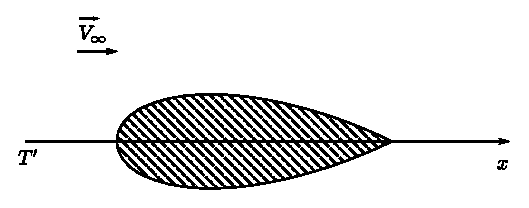
\includegraphics{vol65-figures/fig65-3.1_1.eps}}
\caption{}\label{c4:fig3.1}
\end{figure}


In the\pageoriginale remainder of Sec. 3 (and also in Chap. 6) we
shall only work in the physical plane since it seems more convenient
for the computation of non-symmetric and/or \textit{transonic flows.} 
\end{remark}

For the reader who is interested by the mathematical aspects of the
flow mentioned above, see BERS [\ref{k11:e1}], BREZIS-STAMPACCHIA
[\ref{k16:e1}]. For the 
Physical and Mechanical aspects see LANDAU-LIPSCHITZ [1]. Additional
references are given in Chap. 6.  

\subsection{Variational formulation of subsonic problems}\label{c4:ss3.2}

\textbf{Preliminary Remark:} In the case of a non symmetric flow past
an airfoil (see Figure \ref{c4:fig3.2}) 

\begin{figure}[H]
\centering{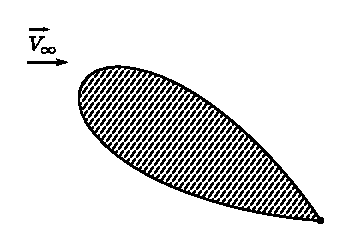
\includegraphics{vol65-figures/fig65-3.2.eps}}
\caption{}\label{c4:fig3.2}
\end{figure}

\noindent the velocity\pageoriginale  potential has to be \textit{discontinuous
  and a circulation condition} is required to ensure the uniqueness
(modulo a constant) of the solution of \eqref{c4:eq3.1}. If the
airfoil has corners (like in Figure \ref{c4:fig3.1}) then the circulation
condition is related to the so called \textit{Kutta-Joukowsky
  condition} from which it follows that for a physical flow, the
velocity field is continuous at the (like 0 in Figure
\ref{c4:fig3.2}). For more information about the Kutta-Joukowsky condition, see
LANDAU-LIPSCHITZ [1] (see also Chap. 6). 

For the sake of simplicity, we shall assume in the sequel that either
$\Omega$ is simply connected, as it is the case for the nozzle of
Figure \ref{c4:fig3.3}, or, if $\Omega$ is multiply connected, we shall assume
(like in Fig. \ref{c4:fig3.1}) that the flow is physically and geometrically
symmetric, since in this case the Kutta-Joukowsky condition is
automatically satisfied. 

\begin{figure}[H]
\centering{\includegraphics{vol65-figures/fig65-3.3.eps}}
\caption{}\label{c4:fig3.3}
\end{figure}


We assume in the sequel that the boundary condition associated with
\eqref{c4:eq3.1}, \eqref{c4:eq3.2} are the following: 
\begin{equation}
\phi = g_0 \text{ over } \Gamma_0, ~\rho \frac{\partial \phi}{\partial
  n}|_{\Gamma_{1}} = g_1 \tag{3.4}\label{c4:eq3.4} 
\end{equation}
where $\Gamma_0$, $\Gamma_1 \subset \Gamma$ with $\Gamma_0 \cap
\Gamma_1 = \phi$, $\Gamma_0 \cup \Gamma_1 = \Gamma$. Then the
variational formulation for the flow problem \eqref{c4:eq3.1},
\eqref{c4:eq3.2}, \eqref{c4:eq3.3}, \eqref{c4:eq3.4} is  
\begin{equation}
\begin{cases}
\int_\Omega \rho (\phi) \nabla \phi \cdot \nabla v dx =
\int_{\Gamma_{1}} g_1 v d \Gamma\, \forall v \in V_0, \\ 
&\\
\phi \in V_{g_{0}},
\end{cases}\tag{3.5}\label{c4:eq3.5}
\end{equation}\pageoriginale 
where 
\begin{align}
& V_0 = \{v \in H^1(\Omega) : v|_{\Gamma_0} = 0\}, \tag{3.6}\label{c4:eq3.6}\\
& V_{g_0} = \{ v \in H^1 (\Omega) : v|_{\Gamma_0} =
  g_0\}. \tag{3.7}\label{c4:eq3.7} 
\end{align}

If $g_0$, $g_1$ are small enough, it can be proved that
\eqref{c4:eq3.5} has a solution such that  
$$
|\nabla \phi| \leq M < C_* \text{ a.e. }.
$$

When solving a practical flow problem we may not know a priori,
whether the flow will be purely subsonic or not. Therefore instead of
solving \eqref{c4:eq3.5} it may be convenient to consider (and solve)
the following problem:  
\begin{equation}
\begin{cases}
\int_\Omega \rho (\phi) \nabla \phi \cdot \nabla (v - \phi) dx \geq \int_{\Gamma_{1}} g_1(v - \phi) d \Gamma\, \forall v \in K_\delta,\\
&\\
\phi \in K_\delta,
\end{cases}\tag{3.8}\label{c4:eq3.8}
\end{equation}
where 
\begin{equation}
K_\delta = \{v \in V_{g_0}, |\nabla v| \leq \delta < C_* a. e. \}. \tag{3.9}\label{c4:eq3.9}
\end{equation}

The variational problem \eqref{c4:eq3.8}, \eqref{c4:eq3.9} is an EVI of the first kind, but we have to observe that unlike the EVIs of Chap. 1 and 2, it involves a non-linear partial differential operator, namely $A$ defined by 
$$
A(\phi) = - \nabla \cdot (\rho(\phi) \nabla \phi).
$$

\begin{remark}\label{c4:rem3.2}%rem 3.2
In practical applications we shall take $\delta$ as close as possible to $C_*$. 
\end{remark}

\begin{remark}\label{c4:rem3.3}%rem 3.3
Problem \eqref{c4:eq3.8}, \eqref{c4:eq3.9} appears as a variant of the elasto-plastic 
torsion problem of Chap.~\ref{chap2}, Sec.~\ref{c2:s3}.
\end{remark}

\subsection{Existence and uniqueness properties for the problem
  (3.8).}\label{c4:ss3.3}  

In this\pageoriginale  section we shall assume that Measure
$(\Gamma_0) >0$. To prove that \eqref{c4:eq3.8} is well posed we will
use the following 

\begin{lemma}\label{c4:lem3.1}%lem 3.1
The function $\xi \to -\left(1-
\dfrac{\xi^2}{\frac{\gamma+1}{\gamma-1}C^2_*}\right)^{\gamma/ \gamma-1}$
is convex if $\xi \in[0, C_*]$, concave if $\xi \in [C_*,
  \sqrt{\dfrac{\gamma+1}{\gamma-1}}C_*]$ and strictly convex if $\xi
\in [ 0, C_* [ $. 
\end{lemma}

\begin{exercise}\label{c4:exer3.1}%exe 3.1
Prove Lemma \ref{c4:lem3.1}.

We can now prove 
\end{exercise}

\begin{theorem}\label{c4:thm3.1}%the 3.1
Assume that $\Omega$ is bounded and that $g_0$, $g_1$ are sufficiently
smooth and small. Then \eqref{c4:eq3.8} has a unique solution. 
\end{theorem}

\begin{proof}%pro
Since $\Omega$ is bounded and if $g_0$ is sufficiently smooth and
small, we observe that $K_\delta$ is a closed, convex, and nonempty
bounded subset of $H^1(\Omega)$ (consisting of uniformly Lipschitz
continuous functions). 

Define $J(\cdot)$ by 
\begin{equation}
J(v) = - \frac{\gamma+ 1}{2 \gamma} C^2_* \int_\Omega \left(1- \frac{|
  \nabla v|^2}{\frac{\gamma + 1}{\gamma - 1}C^2_*}\right)^{\gamma /\gamma -
  1}dx - \int_{\Gamma_1} g_1 v d \Gamma. \tag{3.10}\label{c4:eq3.10} 
\end{equation}
\end{proof}

It follows from Lemma~\ref{c4:lem3.1} that $J(\cdot)$ is strictly convex over $K_\delta$. It is easy to check that $J(\cdot)$ is continuous and Gateau-differentiable over $K_\delta$ with 
\begin{equation}
(J'(v), w) = \int_\Omega \rho (v) \nabla v \cdot \nabla w dx - \int_{\Gamma_1} g_1 w d \Gamma. \tag{3.11}\label{c4:eq3.11}
\end{equation}

Since $K_\delta$ is a closed, convex, nonempty subset of $H^1(\Omega)$ and that $J(\cdot)$ is continuous and strictly convex over $K_\delta$, it follows from standard optimization theory in Hilbert space (see CEA [1], [2]) that the minimization problem 
\begin{equation}
\begin{cases}
J(u) \leq J(v)\, \forall v \in K_\delta, \\
&\\
u \in K_\delta,
\end{cases}\tag{3.12}\label{c4:eq3.12}
\end{equation}
has a unique solution.

Moreover\pageoriginale  since $J(\cdot)$ is differentiable the unique
solution of \eqref{c4:eq3.12} is characterised (see CEA
[\ref{k27:e1}], [\ref{k27:e2}])  by  
\begin{equation*}
\begin{cases}
(J'(u), v-u) \geq 0\, \forall v \in K_\delta,\\
&\\
u \in  K_\delta ;
\end{cases}
\end{equation*}
from \eqref{c4:eq3.11}, this completes the proof of the Theorem. 

\begin{remark}\label{c4:rem3.4}%rem 3.4
Let us assume that $\Gamma_0 = \phi$. Then defining  $K_\delta$ by 
$$
K_\delta = \{v \in H^1(\Omega) : |\nabla v| \leq \delta < C_* a.e.,
v(x_0) = v_0\} 
$$
with $x_0 \in \overline{\Omega}$ and $v_0$ arbitrarily given, we can prove that if $\Omega$ is bounded and $g_1$ is sufficiently smooth then 
\begin{equation}
\begin{cases}
\int_\Omega \rho (\phi) \nabla \phi \cdot \nabla (v -\phi) dx \geq \int_\Gamma g_1 (v-\phi) d\Gamma\, \forall v \in K_\delta\\
&\\
\phi \in K_\delta,
\end{cases}\tag{3.13}\label{c4:eq3.13}
\end{equation}
has a unique solution (if $\phi$ is a solution of \eqref{c4:eq3.13} then $\phi + C$ is the unique solution of the similar problem obtained by replacing $v_0$ by $v_0 +C$).
\end{remark}

\begin{exercise}\label{c4:exer3.2}%exe 3.2
Prove the statement of Remark~\ref{c4:rem3.4}.
\end{exercise}
\begin{remark}\label{c4:rem3.5}%rem 3.5
In all the above arguments we assumed that $\Omega$ is boun\-ded. We
refer to CIAVALDINI-POGU-TOURNMINE [\ref{k36:e1}] in which one carefully studies
the approximation of subsonic flow problems on an unbounded domain
$\Omega_\infty$ by problems on a family $(\Omega_n)_n$ of bounded
domains converging to $\Omega_\infty$ (actually they have obtained
estimates for $\phi_\infty -\phi_n$). 
\end{remark}

The above EVI's will have a practical interest if we can prove that in
the cases where a purely subsonic solution exists, then for $\delta$
large enough it is the solution of \eqref{c4:eq3.8}; actually this
property is true and follows from  

\begin{theorem}\label{c4:thm3.2}%the 3.2
Assuming\pageoriginale  the same hypothesis on $\Omega$, $g_0$, $g_1$
as in Theorem \ref{c4:thm3.1}, and that \eqref{c4:eq3.4} has a unique
solution in $H^1(\Omega)$ with  
\begin{equation}
|\nabla \phi| \leq \delta _0 < C_* \text{ a.e. } \tag{3.14}\label{c4:eq3.14}
\end{equation}
then $\phi$ is a solution of \eqref{c4:eq3.8}, \eqref{c4:eq3.9}
$\forall \delta \in [\delta_0, C_*[$. Conversely if the solution of
    \eqref{c4:eq3.8}, \eqref{c4:eq3.9} is such that $|\nabla
    \phi| \leq \delta_0 < \delta$ a.e., then $\phi$ is a solution of
    \eqref{c4:eq3.1}, \eqref{c4:eq3.2}, \eqref{c4:eq3.4}. 
\end{theorem}

\begin{proof}%pro
\begin{enumerate}[(1)]
\item Let $\phi \in H^1(\Omega)$ satisfying \eqref{c4:eq3.1}, \eqref{c4:eq3.2}, \eqref{c4:eq3.4} and \eqref{c4:eq3.14}. If $v \in V_0$ then using Green's formula it follows from \eqref{c4:eq3.1}, \eqref{c4:eq3.2}, \eqref{c4:eq3.4} that 
\begin{equation}
\int_\Omega \rho(\phi) \nabla \phi \cdot \nabla v dx = \int_{\Gamma_1} g_1 v d\Gamma\, \forall v \in V_0. \tag{3.15}\label{c4:eq3.15}
\end{equation}
It follows from \eqref{c4:eq3.4}, \eqref{c4:eq3.15} and from the definition of $V_{g_0}$ that 
\begin{equation}
\int_\Omega \rho (\phi) \nabla \phi \cdot \nabla (v-\phi) dx = \int_{\Gamma_{1}} g_1 (v-\phi) d \Gamma\, \forall v \in V_{g_0}. \tag{3.16}\label{c4:eq3.16}
\end{equation}
Since $\phi \in K_\delta \subset V_{g_0}\, \forall \delta \in [\delta_0, C_*[$, it follows from \eqref{c4:eq3.16} that 
\begin{equation*}
\begin{cases}
\int_\Omega \rho (\phi) \nabla \phi \cdot \nabla (v -\phi) dx \geq \int_\Gamma g_1 (v-\phi) d\Gamma\, \forall v \in K_\delta, \\
&\\
\phi \in K_\delta,
\end{cases}
\end{equation*}
if $\delta \in [\delta_0, C_*[$; therefore $\phi$ is the solution of the EVI \eqref{c4:eq3.8}, \eqref{c4:eq3.9} $\forall \delta \in [\delta_0, C_*[$.
\item Define $U \subset V_0$ by 
$$
U = \{v \in C^\infty (\overline{\Omega}) : v =0 \text{ in a neighbourhood of  }\Gamma_0\}.
$$
\end{enumerate}
\end{proof}
Then, if we suppose that $\Gamma$ is sufficiently smooth, we have 
\begin{equation}
\overline{U}^{H^1(\Omega)} = V_0. \tag{3.17}\label{c4:eq3.17}
\end{equation}
We assume that for $\delta < C_*$, \eqref{c4:eq3.8} has a solution such that 
\begin{equation}
|\nabla \phi| \leq \delta_0 < \delta \text{ a.e. }. \tag{3.18}\label{c4:eq3.18}
\end{equation}\pageoriginale 

Then $\forall v \in U$ and for $t> 0$ sufficiently small $\phi + tv
\in K_\delta$. Then replacing $v$ by $\phi + tv$ in \eqref{c4:eq3.8}
and dividing by $t$ obtain 
$$
\int_\Omega \rho (\phi) \nabla \phi \cdot \nabla v dx \geq \int
_{\Gamma_1} g_1 v d \Gamma\, \forall v \in U, 
$$
which implies 
\begin{equation}
\int_\Omega \rho (\phi) \nabla \phi \cdot \nabla v dx = \int _{\Gamma_1} g_1 v d \Gamma\, \forall v \in U. \tag{3.19}\label{c4:eq3.19}
\end{equation}
Since $\mathscr{D}(\Omega) \subset U$ it follows from \eqref{c4:eq3.19} that 
\begin{equation}
\int_\Omega \rho (\phi) \nabla \phi \cdot \nabla v dx = 0\, \forall v \in \mathscr{D}(\Omega), \tag{3.20}\label{c4:eq3.20}
\end{equation}
i.e.
$$
-\nabla \cdot (\rho (\phi) \nabla \phi) = 0
$$
which proves \eqref{c4:eq3.1}.

Assuming \eqref{c4:eq3.1} and Green's formula we obtain
\begin{equation}
\int_\Omega \rho (\phi) \nabla \phi \cdot \nabla v dx = \int _{\Gamma_{1}} \rho \frac{\partial \phi}{\partial n} v d \Gamma\, \forall v \in U. \tag{3.21}\label{c4:eq3.21}
\end{equation}
Using \eqref{c4:eq3.17} and comparing with \eqref{c4:eq3.19} we obtain 
$$
\rho \frac{\partial \phi}{\partial n}|_{\Gamma_1} = g_1,
$$
i.e. \eqref{c4:eq3.4}, which completes the proof of the Theorem.

\begin{remark}\label{c4:rem3.6}%rem 3.6
A similar Theorem can be proved for the problem mentioned in 
Remark~\ref{c4:rem3.4}.
\end{remark}

\subsection{Comments}\label{c4:ss3.4}

The solution of subsonic flow problems via EVIs like \eqref{c4:eq3.8}
\eqref{c4:eq3.13} is considered in CIAVALDINI-POGU-TOURNEMINE [\ref{k36:e2}]
(using a stream function approach) and in GLOWINSKI-MARROCCO [\ref{k54:e3}]. 

Iterative methods for solving these EVIs may be found in the above 
reference and also in Chap.~\ref{chap5} of these notes. 
